\section{Aplicação a Dados Simulados}

% Nesta seção, avalia-se o desempenho do modelo proposto GG-KM em diferentes cenários de simulação, com o
% objetivo de investigar sua capacidade de adaptação sob diferentes estruturas do componente de
% cura. Para isso, foram considerados dois tamanhos de amostra ($n=300$ e $n=600$) e três métodos
% para geração de dados, representando diferentes relações entre covariáveis e fração de cura.

% A Figura~\ref{fig:simul_optuna} apresenta a distribuição do IBS para
% cada kernel, obtida ao longo das replicações da validação cruzada. Como medida global de desempenho
% preditivo em análise de sobrevivência, menores valores de IBS indicam melhor ajuste.

% De forma geral, observa-se que a escolha do kernel impacta diretamente a qualidade das estimativas,
% sobretudo em cenários mais complexos. No método 1, o desempenho entre os kernels é relativamente mais
% heterogêneo, com vantagem para kernels como cauchy, exponential e sigmoid,
% que apresentam menores valores centrais de IBS e menor variabilidade.

% Nos métodos 2 e 3, por outro lado, o padrão é mais consistente: kernels não lineares, em especial
% rbf, cauchy, exponential e polynomial, tendem a apresentar melhor
% desempenho e maior estabilidade quando comparados ao kernel linear. Esse comportamento sugere que tais
% cenários envolvem estruturas mais complexas, cuja modelagem é favorecida por espaços de maior
% flexibilidade induzidos por esses kernels.

% Além disso, o aumento do tamanho amostral de $n=300$ para $n=600$ produz uma redução sistemática tanto
% nos níveis quanto na dispersão do IBS, indicando maior estabilidade do processo de estimação e menor erro
% de generalização. Esse resultado reforça a consistência do modelo e evidencia o ganho de eficiência
% associado ao aumento da informação amostral.

% Dessa forma, os resultados mostram que o desempenho do GG-KM é fortemente dependente da especificação do
% kernel, sendo os kernels não lineares particularmente mais adequados em cenários com maior complexidade
% nos dados.

\begin{figure}[htb]
    \centering
    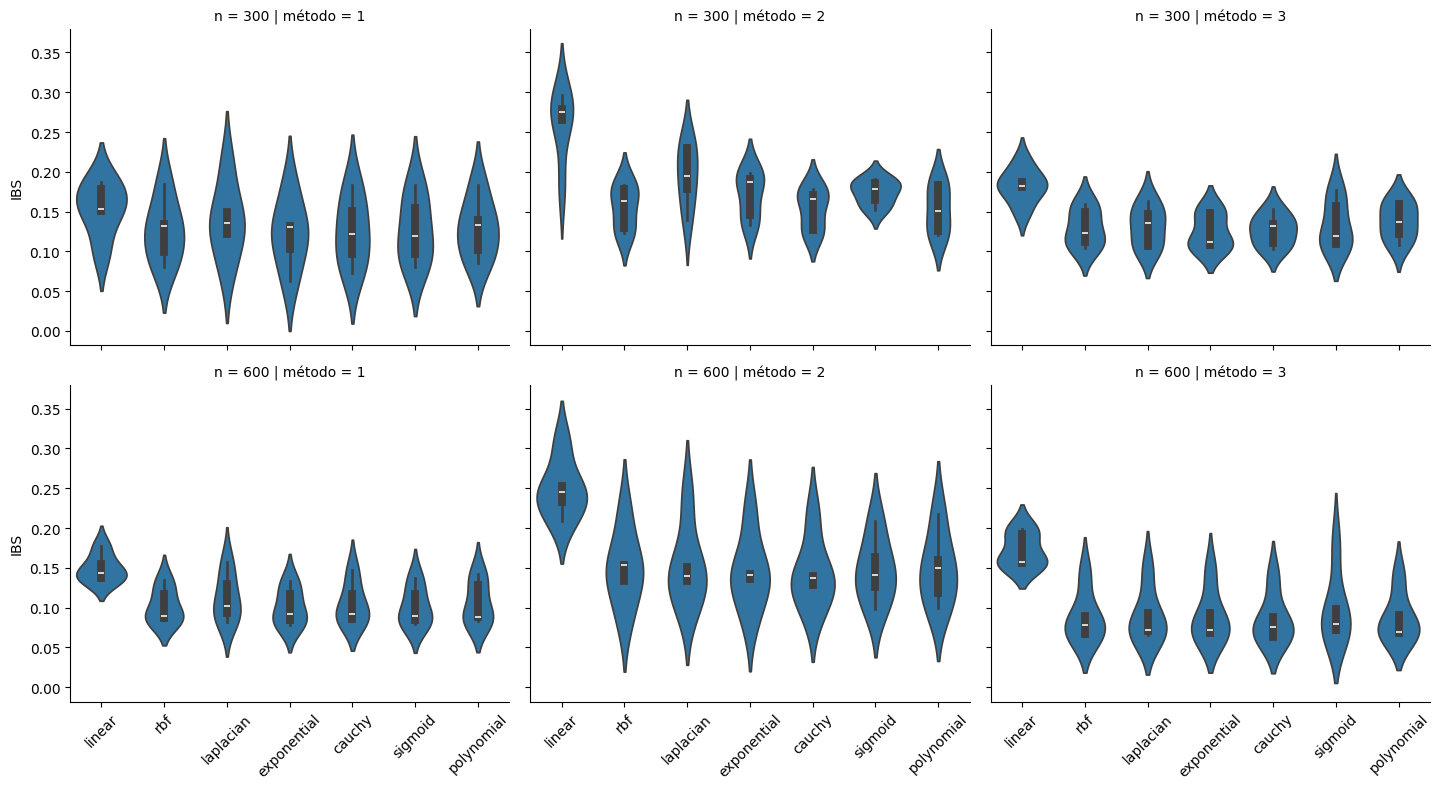
\includegraphics[width=0.8\textwidth]{images/simul_results_violin_em.png}
    \caption{Distribuição do IBS em relação a cada kernel, para diferentes cenários de simulação.}
    \label{fig:simul_optuna}
\end{figure}

% Como indicativo da capacidade do modelo proposto em capturar a fração de cura presente nos dados,
% foi realizada também uma comparação entre o estimador de Kaplan-Meier e a curva de sobrevivência estimada
% pelo modelo GG-KM. Essa comparação pode ser observada na Figura~\ref{fig:km_curv_comparison_ggkm}. De modo
% geral, observa-se que o modelo GG-KM apresenta boa aderência ao comportamento do estimador de Kaplan-Meier,
% sugerindo que o componente de cura está sendo adequadamente modelado. Contudo, no cenário em que $n=600$
% para o método 3, nota-se um afastamento maior entre as curvas, indicando um ajuste inferior nesse caso
% específico.

\begin{figure}[htb]
    \centering
    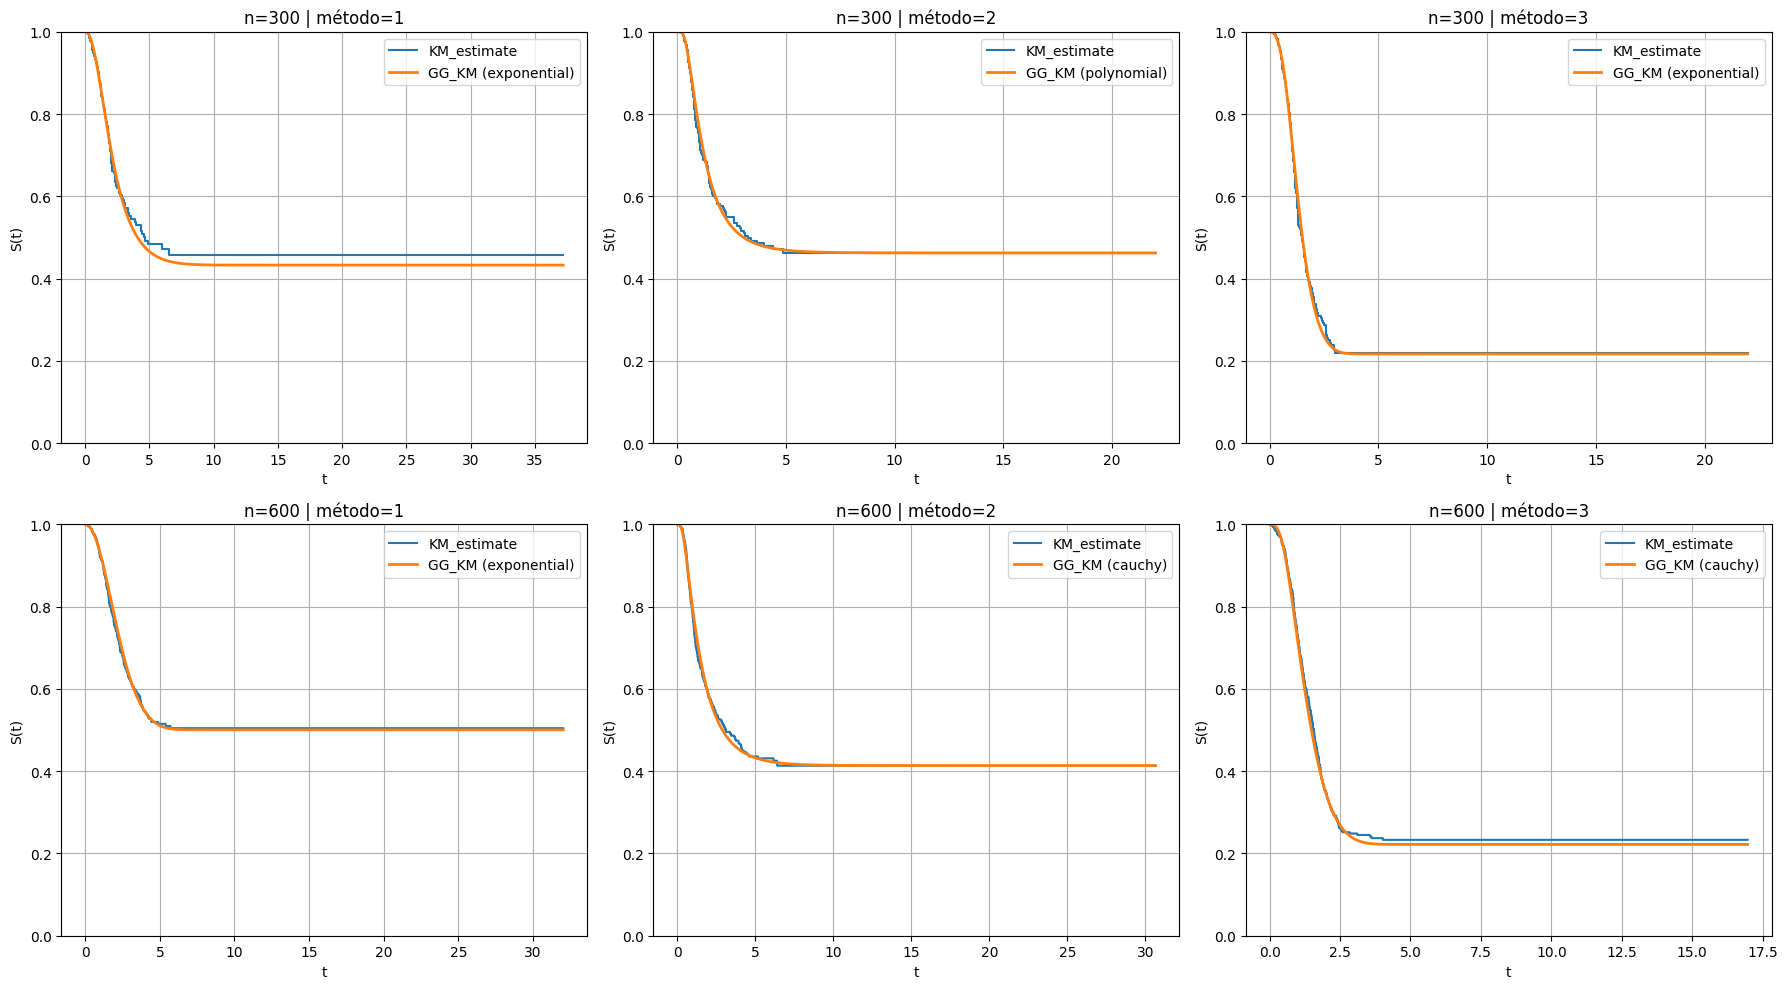
\includegraphics[width=0.8\textwidth]{images/km_curve_comparison_ggkm_em.png}
    \caption{Comparação da curva de sobrevivência estimada pelo GG-KM e KME.}
    \label{fig:km_curv_comparison_ggkm}
\end{figure}

% A Tabela~\ref{tab:resultados_melhores} complementa a análise anterior ao sintetizar, para cada cenário,
% o kernel com melhor desempenho segundo o critério de menor IBS médio. Os resultados reforçam a evidência
% de que kernels não lineares tendem a oferecer melhor capacidade de adaptação às diferentes estruturas
% simuladas.

% Observa-se que o kernel cauchy foi selecionado nos cenários com $n=300$ para os métodos 1 e 2,
% enquanto os kernels exponential, rbf, sigmoid e polynomial também se
% destacaram em diferentes configurações.

% Além disso, nota-se que o aumento do tamanho amostral resultou, em geral, em redução do IBS médio e do viés
% absoluto, especialmente nos métodos 2 e 3, indicando ganhos em precisão e estabilidade na estimação da
% fração de cura. Em particular, o cenário com $n=600$ e método 3 apresentou o melhor desempenho, com
% menor IBS e menor EQM.

\begin{table}[ht]
\centering
\footnotesize
\setlength{\tabcolsep}{3pt}
\caption{Comparação entre as versões Poisson e Binomial Negativa do modelo GG-KM.}
\label{tab:ggkm_comparison}
\begin{tabular}{cc|cccc|cccc}
\toprule
&
&
\multicolumn{4}{c|}{Poisson}
&
\multicolumn{4}{c}{Binomial Negativa - com $\phi$ estimado}
\\
\cmidrule(lr){3-6}
\cmidrule(lr){7-10}
$n$
&
Método
&
$\mathbf{K}$
&
IBS
&
$\text{Viés}\left(\hat{\pi}\left(\mathbf{x}\right)\right)$
&
$\text{EQM}\left(\hat{\pi}\left(\mathbf{x}\right)\right)$
&
$\mathbf{K}$
&
IBS
&
$\text{Viés}\left(\hat{\pi}\left(\mathbf{x}\right)\right)$
&
$\text{EQM}\left(\hat{\pi}\left(\mathbf{x}\right)\right)$
\\
\midrule

\multirow{3}{*}{300}
& 1 & exp. & 0.1221 & -0.0505 & 0.0305
    & exp. & 0.1220 & -0.0443 & 0.0292 \\

& 2 & poly. & 0.1528 & 0.0709 & 0.0778
    & cauchy & 0.1528 & 0.0539 & 0.0706 \\

& 3 & exp. & 0.1248 & -0.0088 & 0.0211
    & exp. & 0.1226 & -0.0039 & 0.0197 \\

\midrule

\multirow{3}{*}{600}
& 1 & exp. & 0.1009 & 0.0100 & 0.0249
    & sigmoid & 0.1008 & 0.0118 & 0.0300 \\

& 2 & cauchy & 0.1429 & -0.0048 & 0.0260
    & exp. & 0.1430 & -0.0046 & 0.0297 \\

& 3 & cauchy & 0.0854 & 0.0052 & 0.0213
    & cauchy & 0.0856 & 0.0052 & 0.0213 \\

\bottomrule
\end{tabular}
\end{table}

% \begin{table}[ht]
% \centering
% \caption{Resultados dos melhores kernels para cada tamanho amostral e método.}
% \label{tab:resultados_melhores}
% \begin{tabular}{ccccccccc}
% \toprule
% n & Método & $\mathbf{K}$ & Média IBS & $\text{Viés}\left(\hat{\pi}\left(\mathbf{x}\right)\right)$ & $\text{EQM}\left(\hat{\pi}\left(\mathbf{x}\right)\right)$ \\
% \midrule
% 300 & 1 & exponential      & 0.1221 & -0.0505 & 0.0305 \\
% 300 & 2 & polynomial      & 0.1528 &  0.0709 & 0.0778 \\
% 300 & 3 & exponential & 0.1248 & -0.0088 & 0.0211 \\
%  \\
% 600 & 1 & exponential     & 0.1009 &  0.0100 & 0.0249 \\
% 600 & 2 & cauchy         & 0.1429 & -0.0048 & 0.0260 \\
% 600 & 3 & cauchy  & 0.0854 & 0.0052 & 0.0213 \\
% \bottomrule
% \end{tabular}
% \end{table}


\section{Aplicação a Dados Reais}

% O conjunto de dados reais escolhido para aplicação do modelo foi o Melanoma, amplamente utilizado em estudos
% de análise de sobrevivência. Esse conjunto contém informações de 205 pacientes diagnosticados com melanoma
% maligno, um tipo agressivo de câncer de pele, submetidos a cirurgia radical no Hospital Universitário de
% Odense, na Dinamarca, entre os anos de 1962 e 1977.

% Os pacientes foram acompanhados até o final de 1977, período no qual 134 indivíduos permaneceram vivos,
% enquanto 71 evoluíram para óbito, sendo 57 mortes atribuídas diretamente ao melanoma e 14 decorrentes de
% outras causas. Este conjunto de dados, especificiamente, é utilizado em textos de modelos com fração de cura,
% pois há o conhecimento de que existe de fato uma fração de cura no conjunto de dados.

% A base é composta por sete variáveis: tempo de acompanhamento em dias (time), status do paciente ao final do estudo (status), sexo
% (sex), idade no momento da cirurgia (age), ano da cirurgia (year), espessura do tumor em milímetros
% (thickness) e presença de ulceração (ulcer).

% Para fins de modelagem, consideramos como evento de interesse o óbito por melanoma, tratando os demais casos,
% pacientes vivos ao final do estudo ou óbitos por outras causas, como observações censuradas. Portanto, ao final,
% tem-se aproximadamente $73\%$ de observações censuradas.

% \begin{figure}[htb]
%     \centering

%     \begin{subfigure}{0.47\textwidth}
%         \centering
%         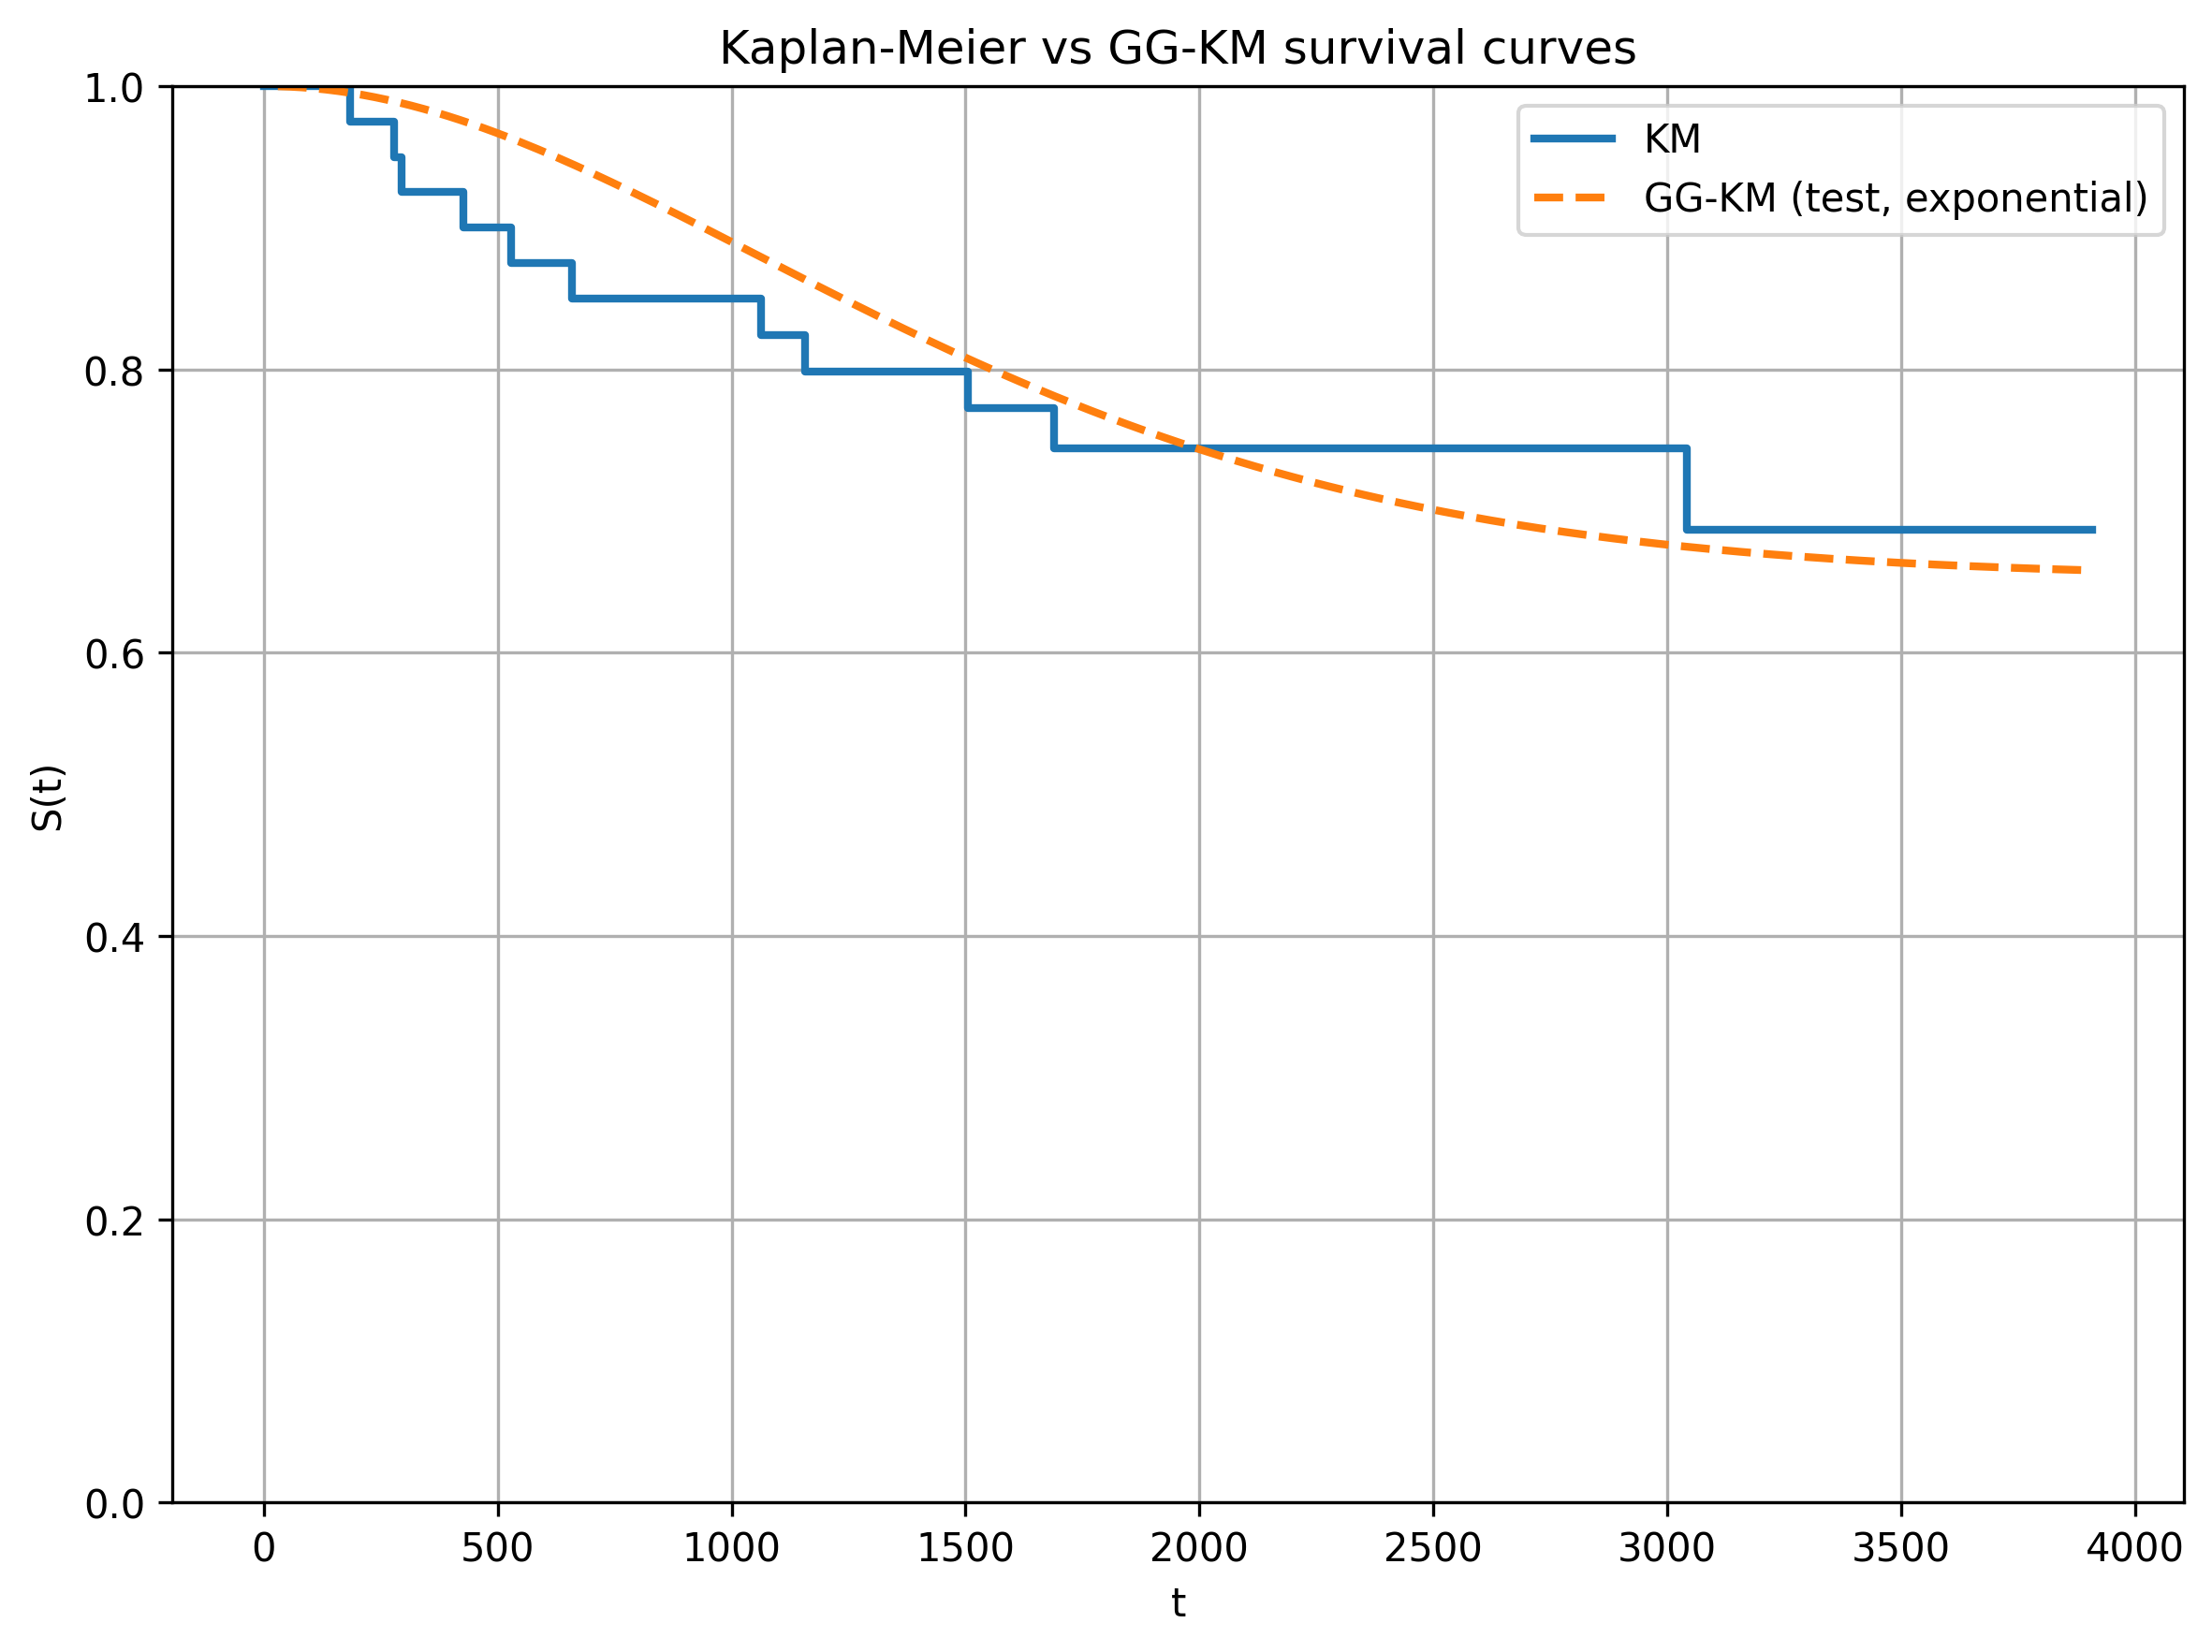
\includegraphics[width=\textwidth]{images/survival_curve_ggkm_testset_bernoulli.png}
%         \caption{Bernoulli}
%     \end{subfigure}
%     \hfill
%     \begin{subfigure}{0.47\textwidth}
%         \centering
%         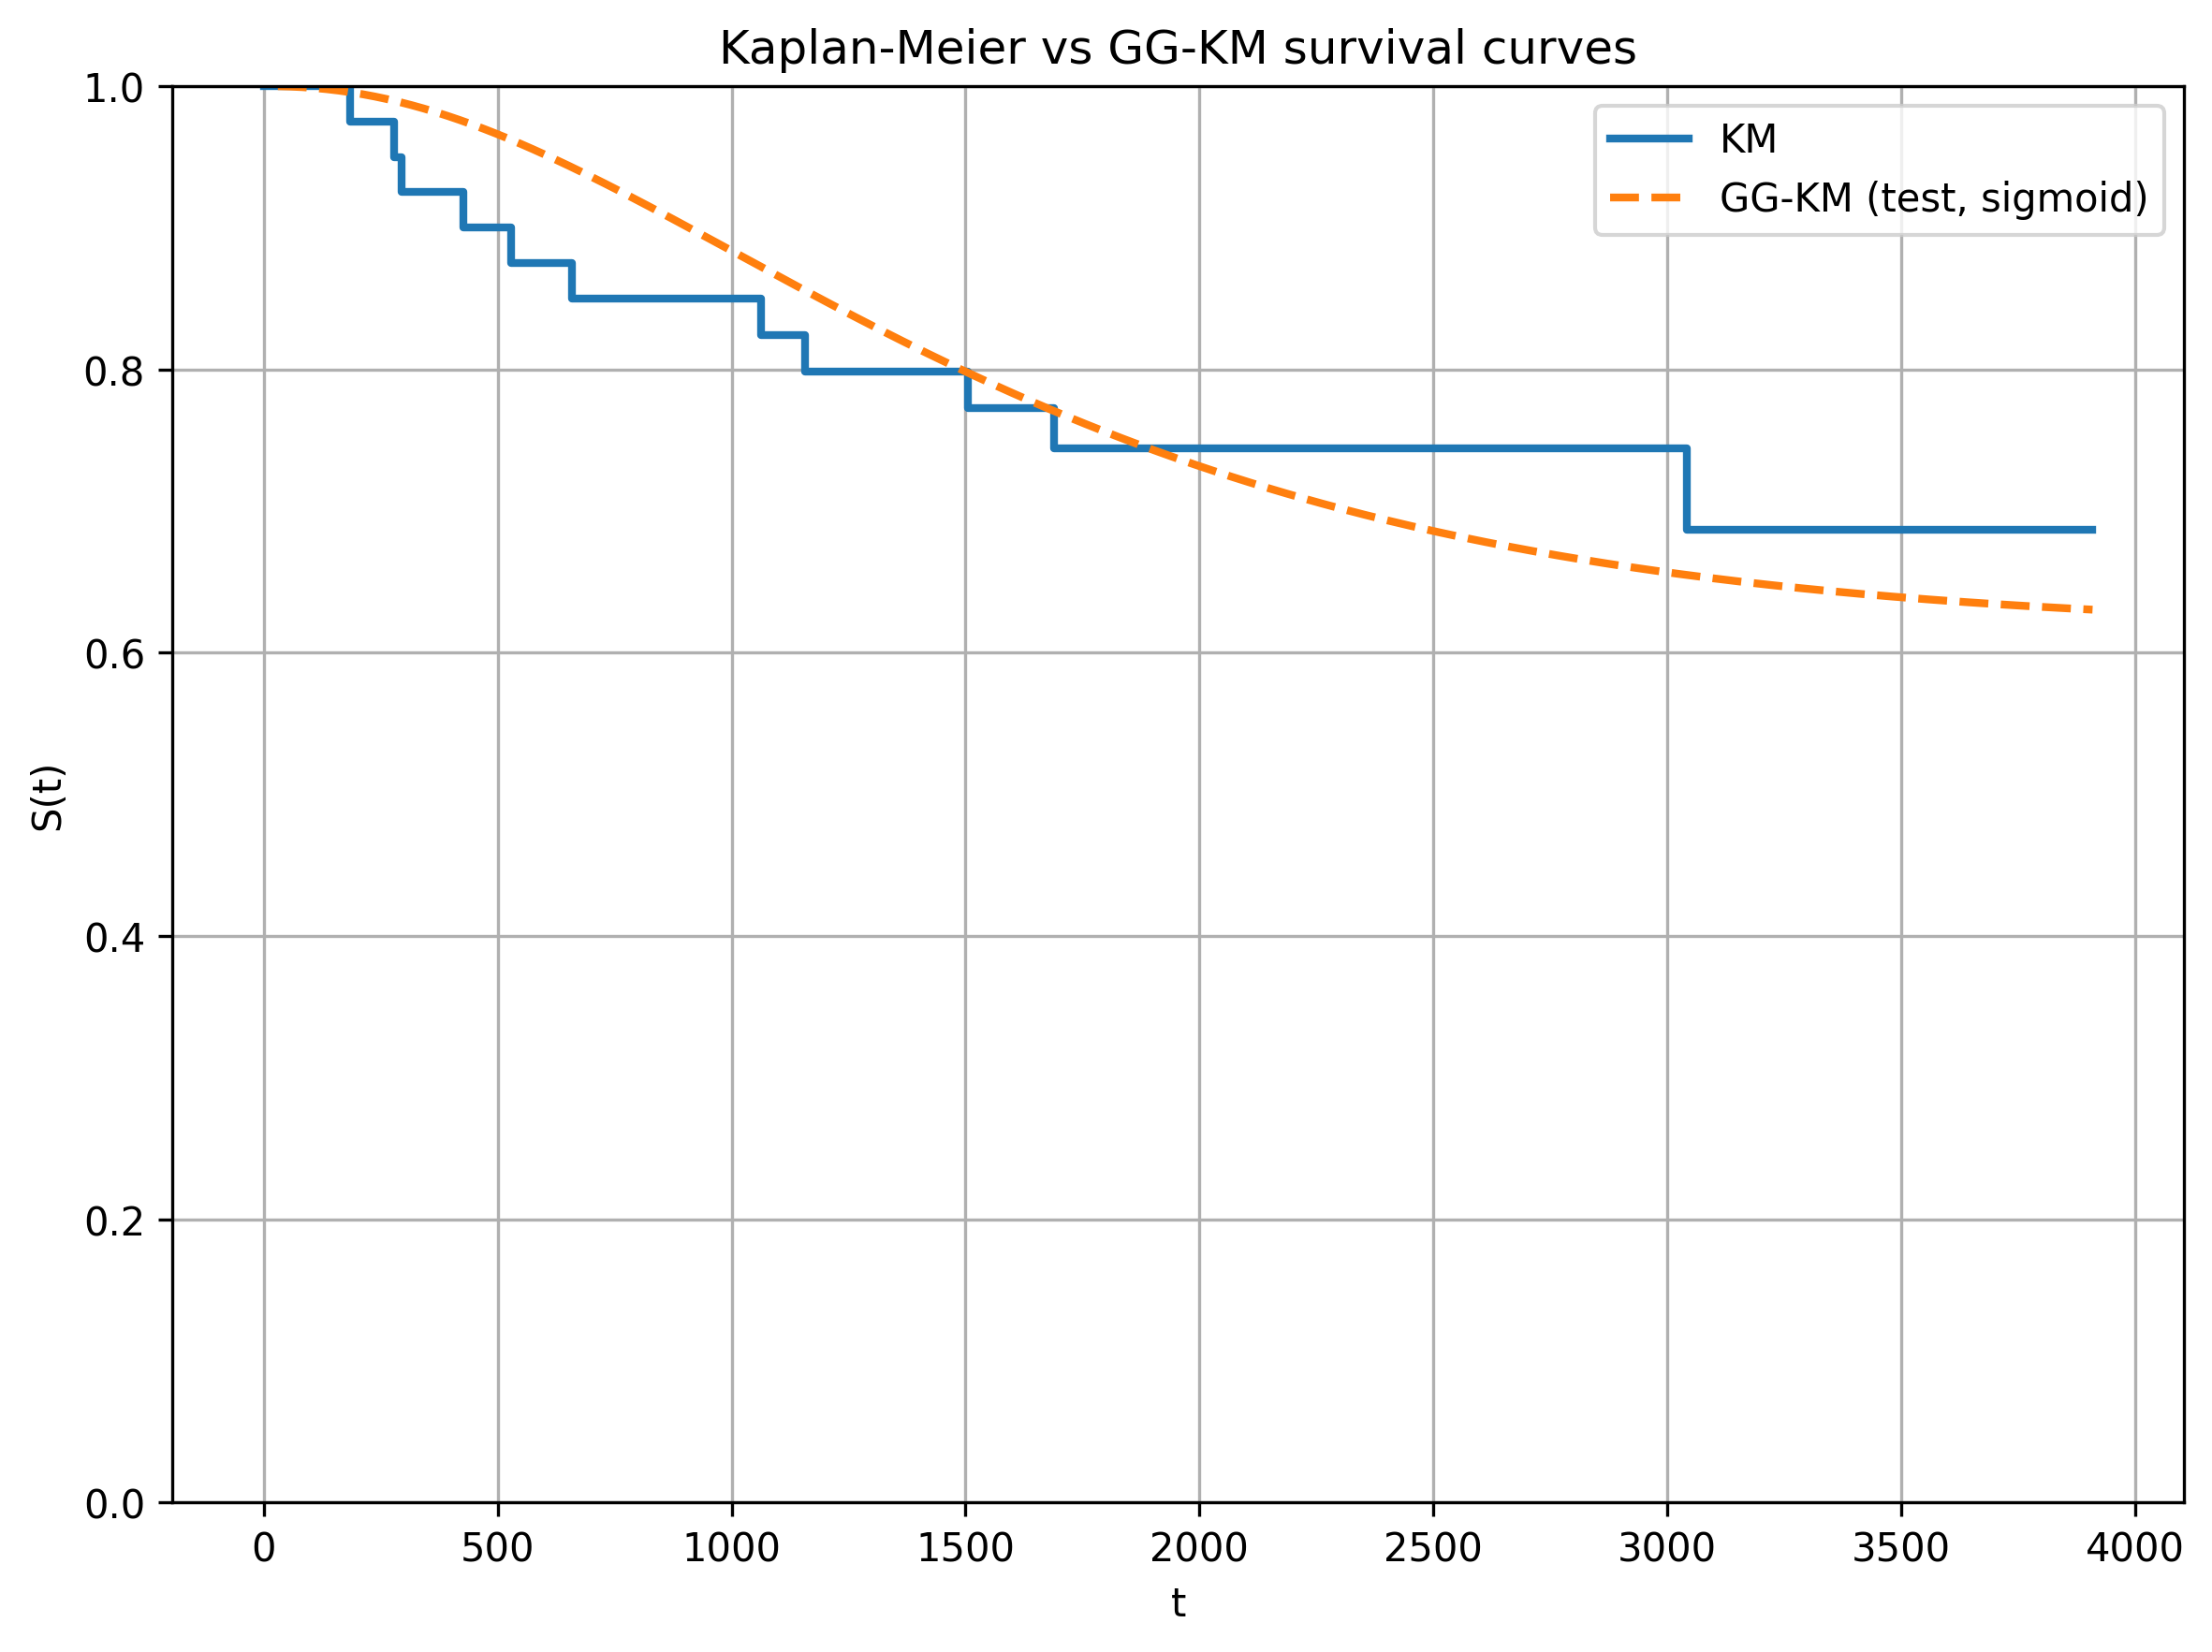
\includegraphics[width=\textwidth]{images/survival_curve_ggkm_testset_binomial.png}
%         \caption{Binomial}
%     \end{subfigure}

%     \vspace{0.3cm}

%     \begin{subfigure}{0.47\textwidth}
%         \centering
%         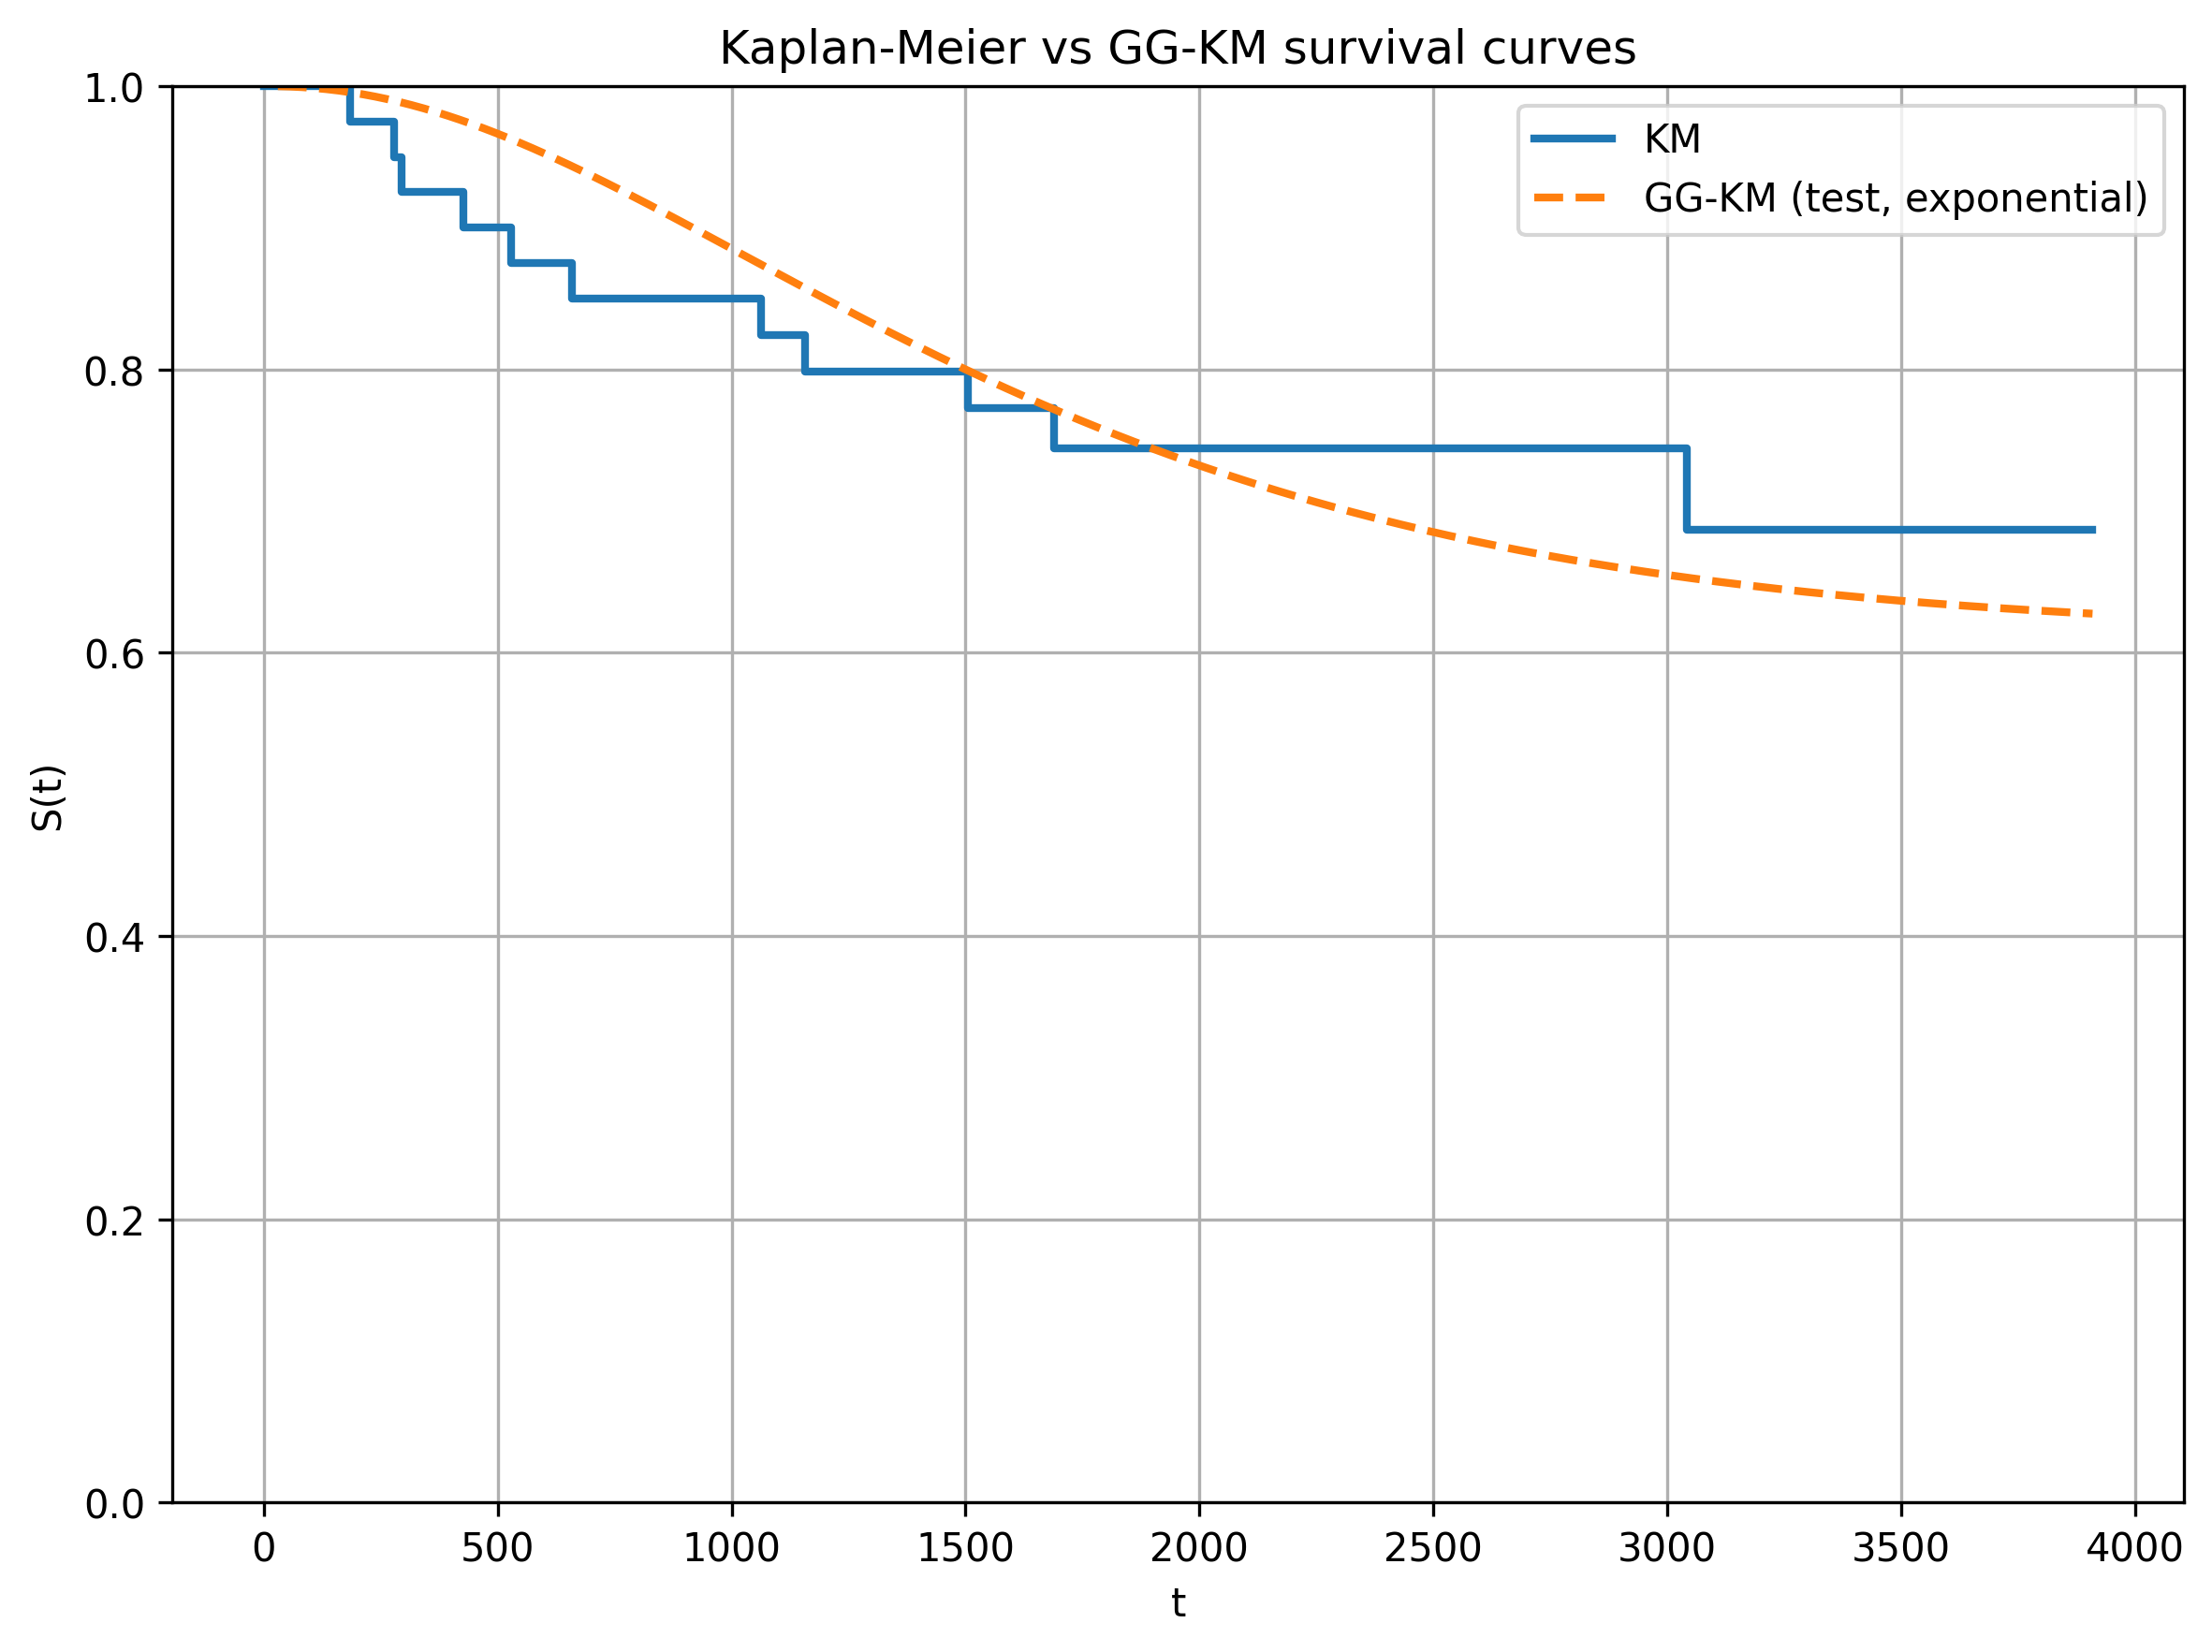
\includegraphics[width=\textwidth]{images/survival_curve_ggkm_testset_poisson.png}
%         \caption{Poisson}
%     \end{subfigure}
%     \hfill
%     \begin{subfigure}{0.47\textwidth}
%         \centering
%         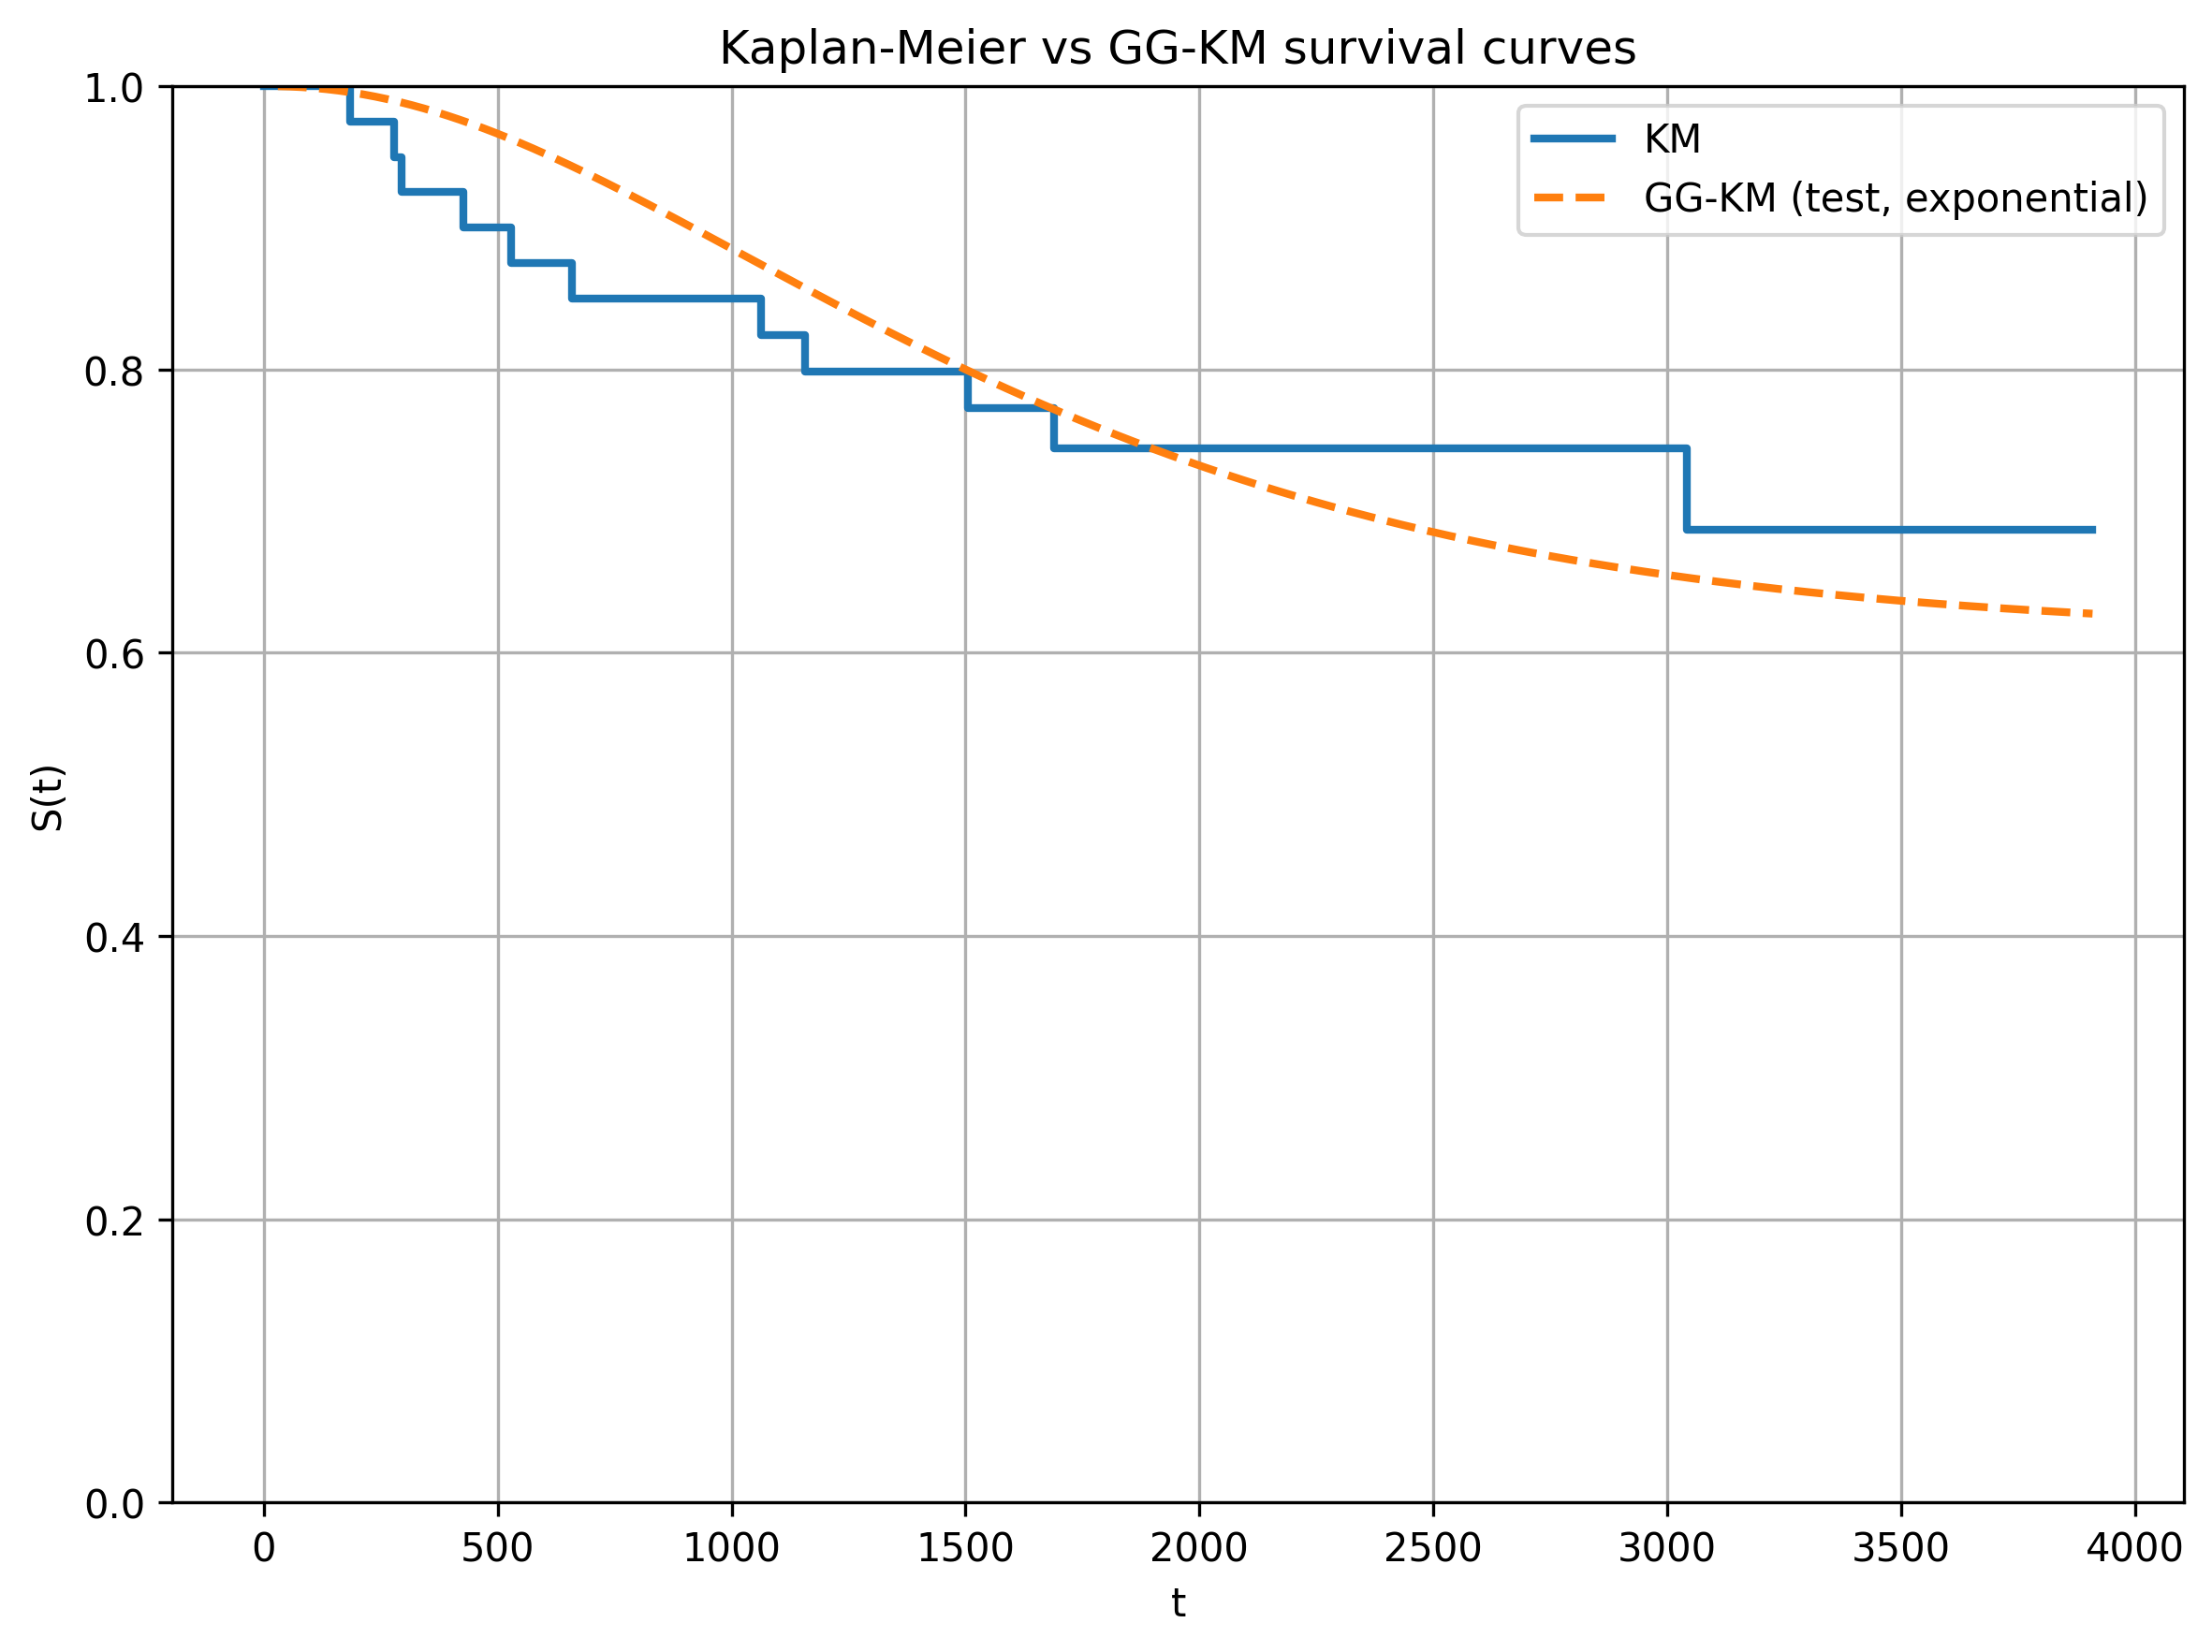
\includegraphics[width=\textwidth]{images/survival_curve_ggkm_testset_bn.png}
%         \caption{Negative Binomial}
%     \end{subfigure}

%     \vspace{0.3cm}

%     \begin{subfigure}{0.47\textwidth}
%         \centering
%         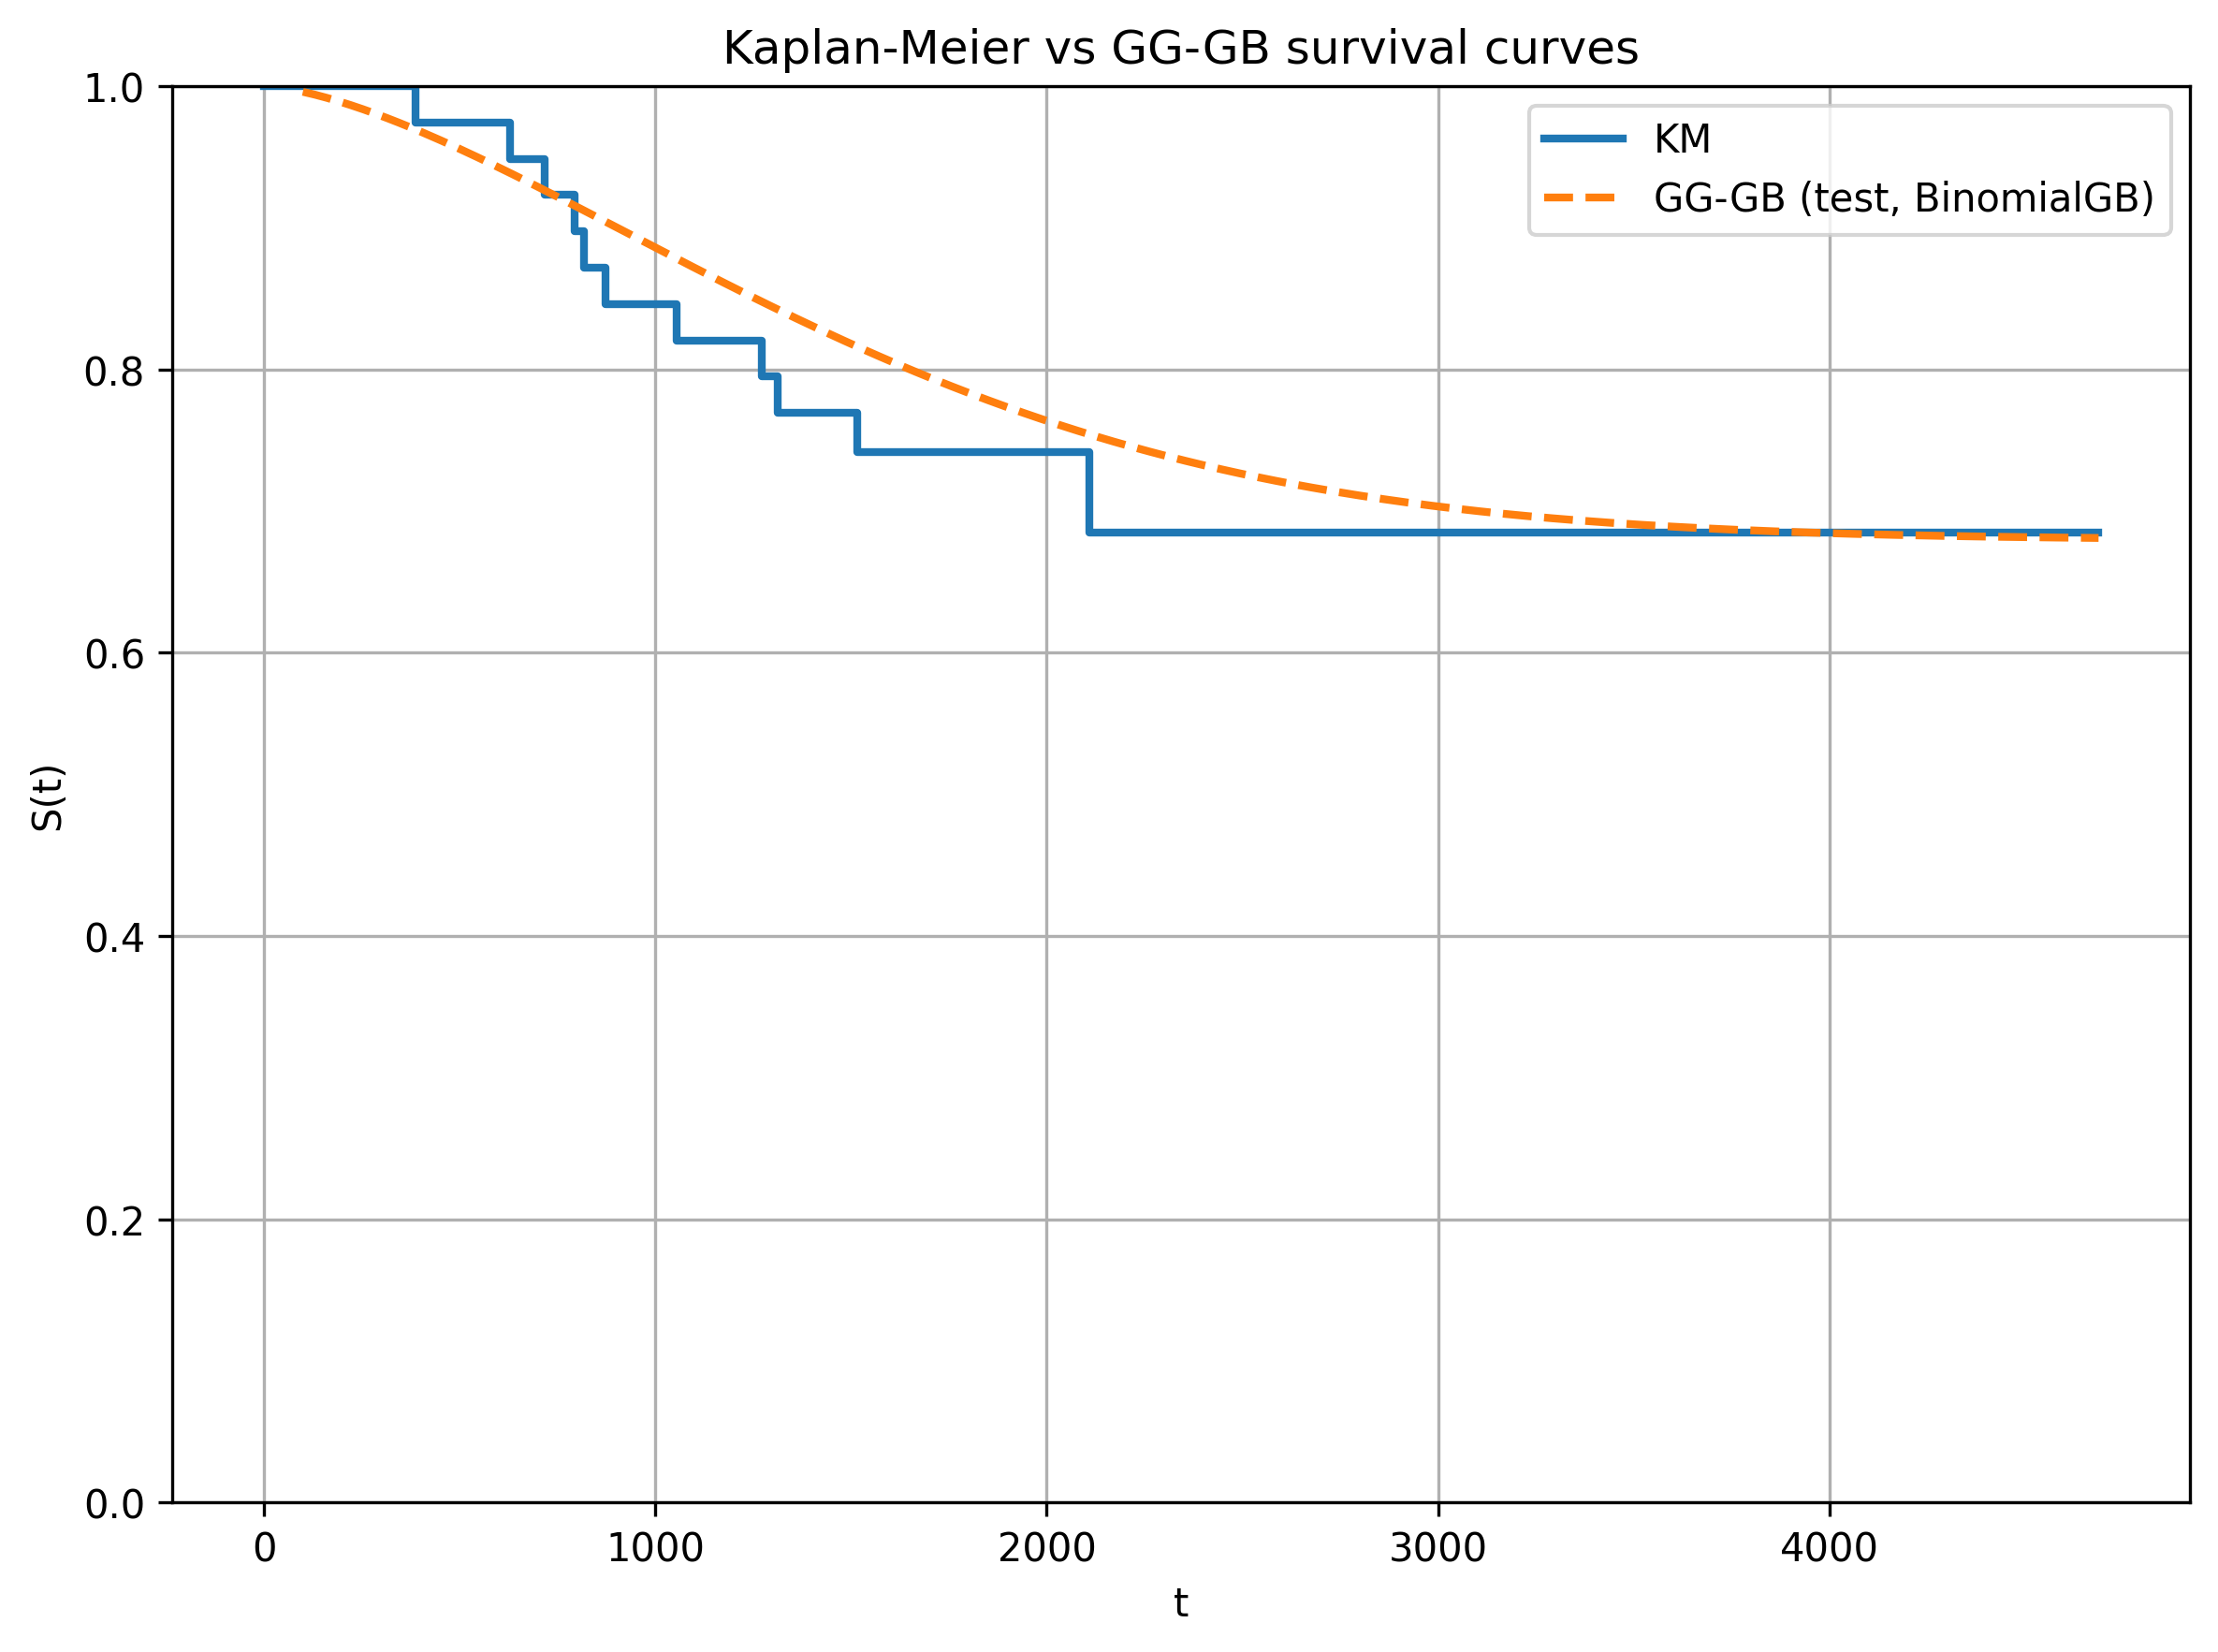
\includegraphics[width=\textwidth]{images/survival_curve_ggkm_testset_boost_bernoulli.png}
%         \caption{Boosted Bernoulli}
%     \end{subfigure}
%     \hfill
%     \begin{subfigure}{0.47\textwidth}
%         \centering
%         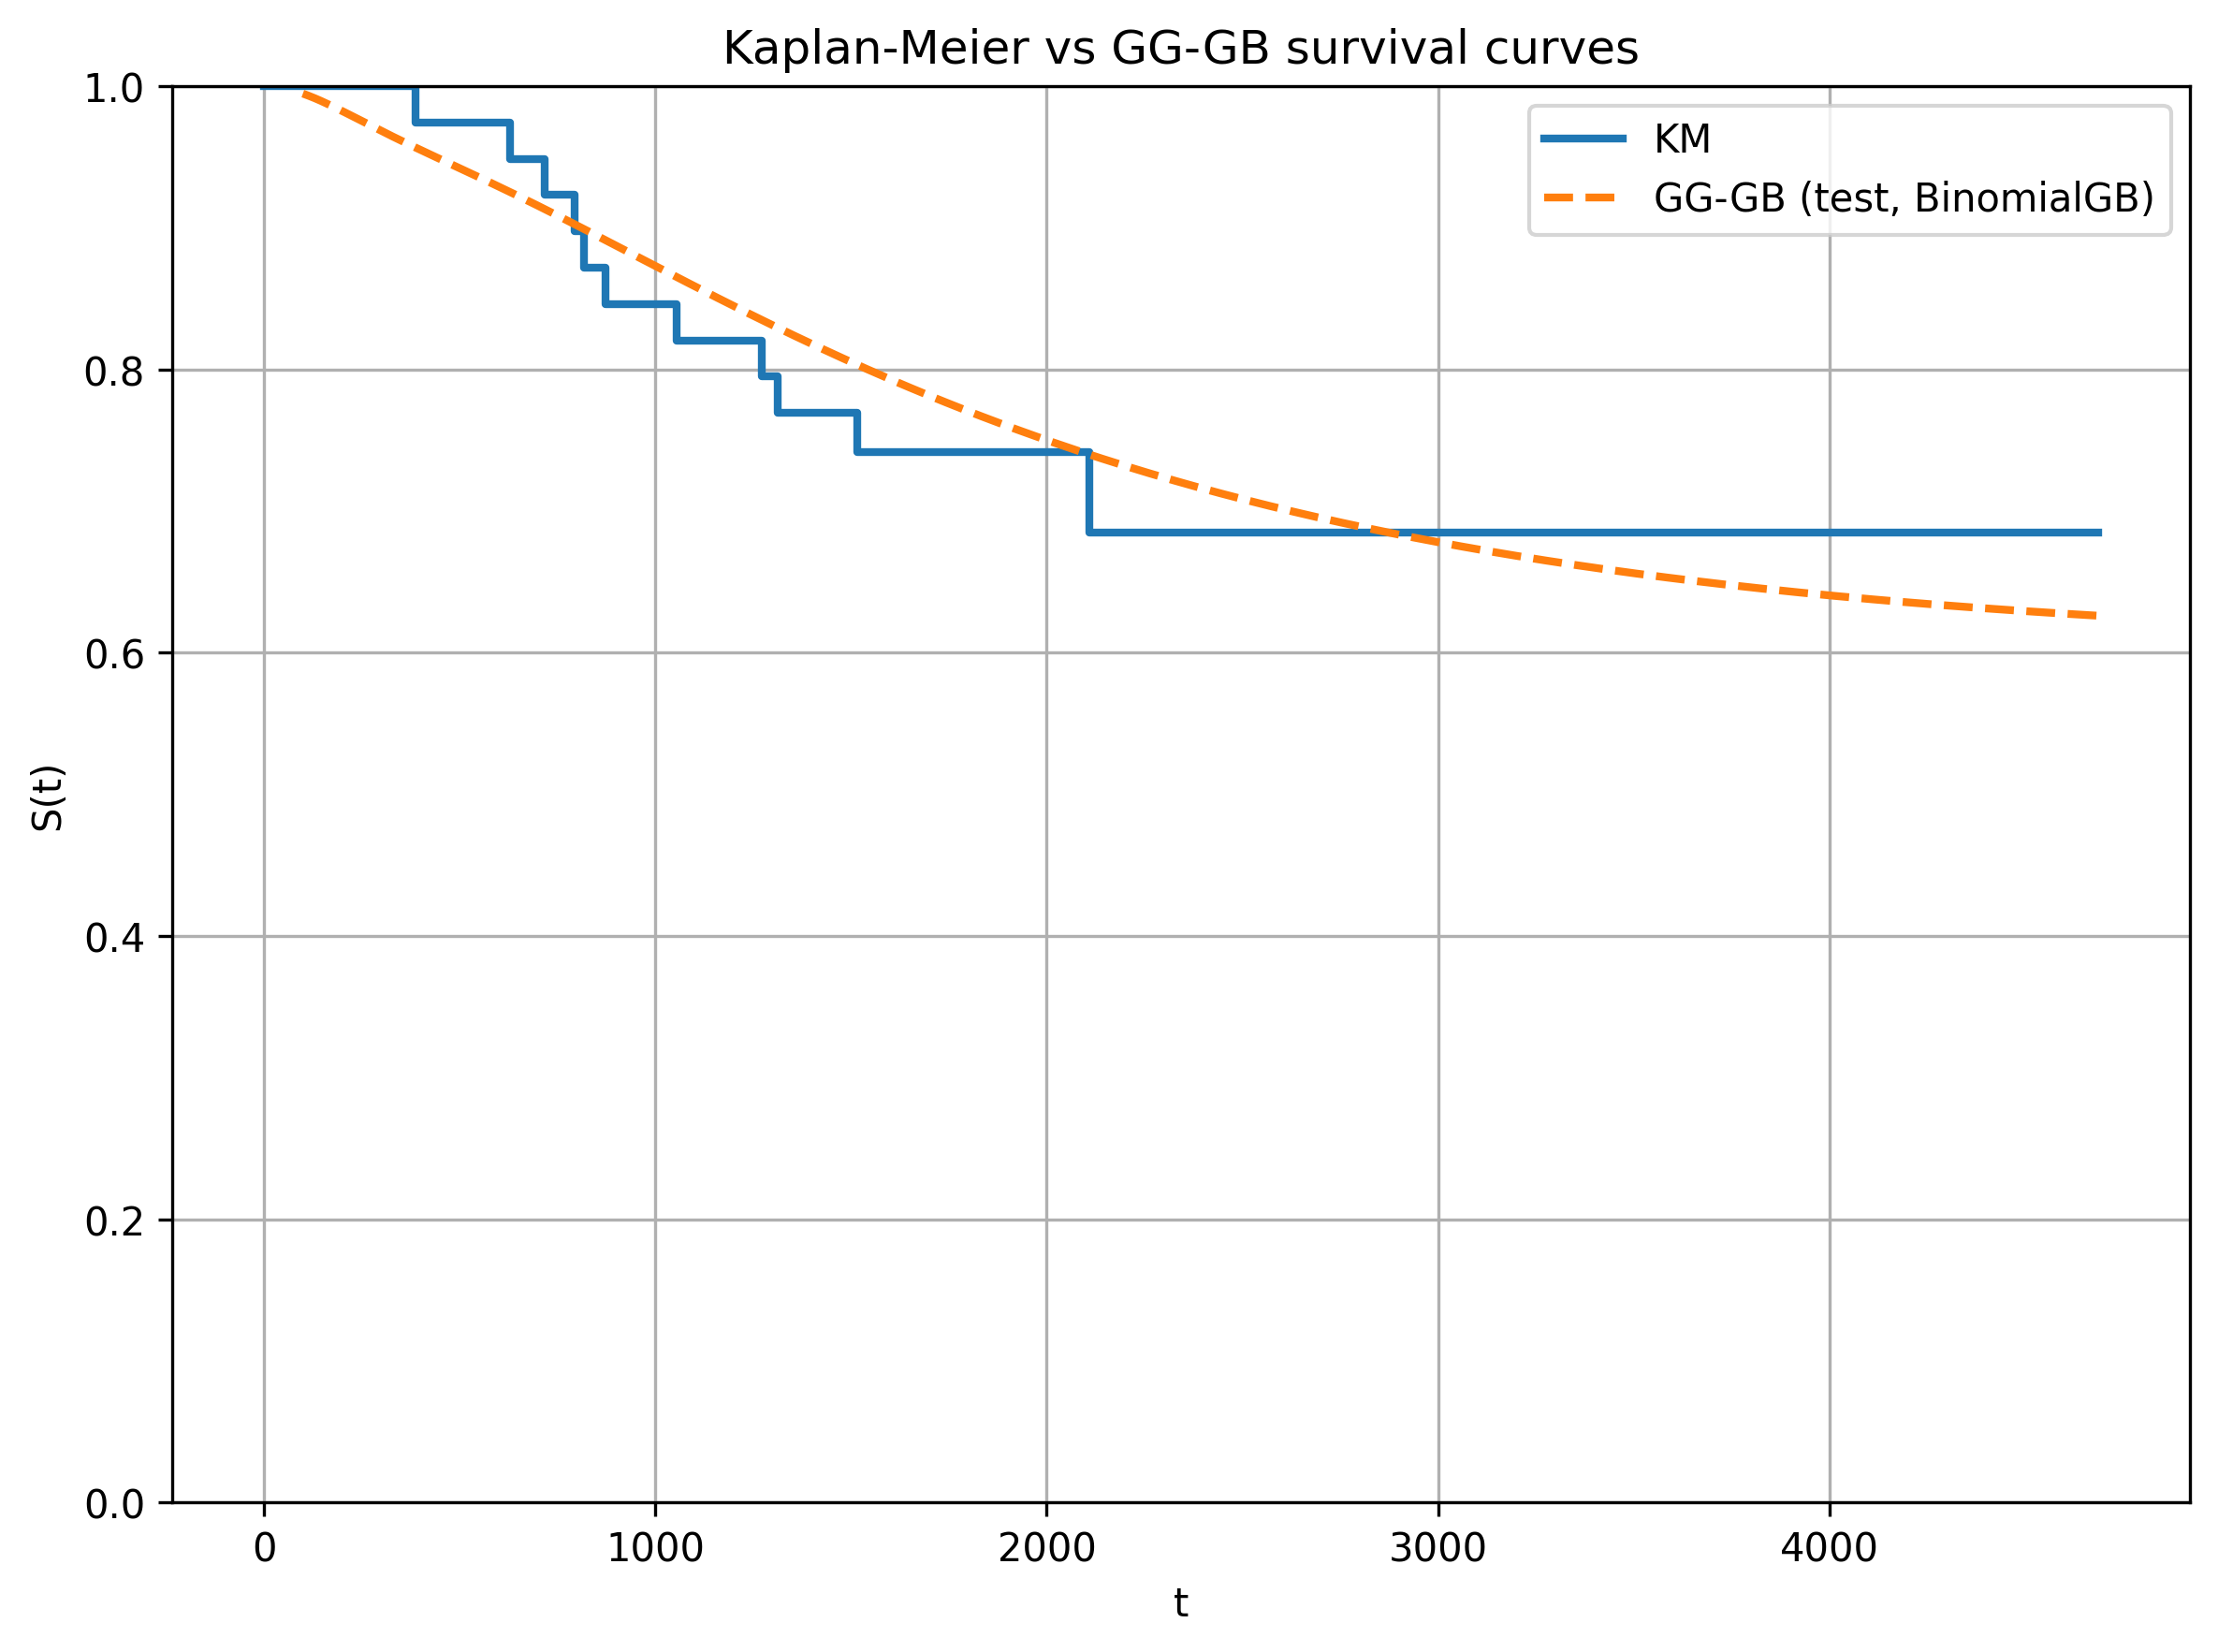
\includegraphics[width=\textwidth]{images/survival_curve_ggkm_testset_boost_binomial.png}
%         \caption{Boosted Binomial}
%     \end{subfigure}

%     \vspace{0.3cm}

%     \begin{subfigure}{0.47\textwidth}
%         \centering
%         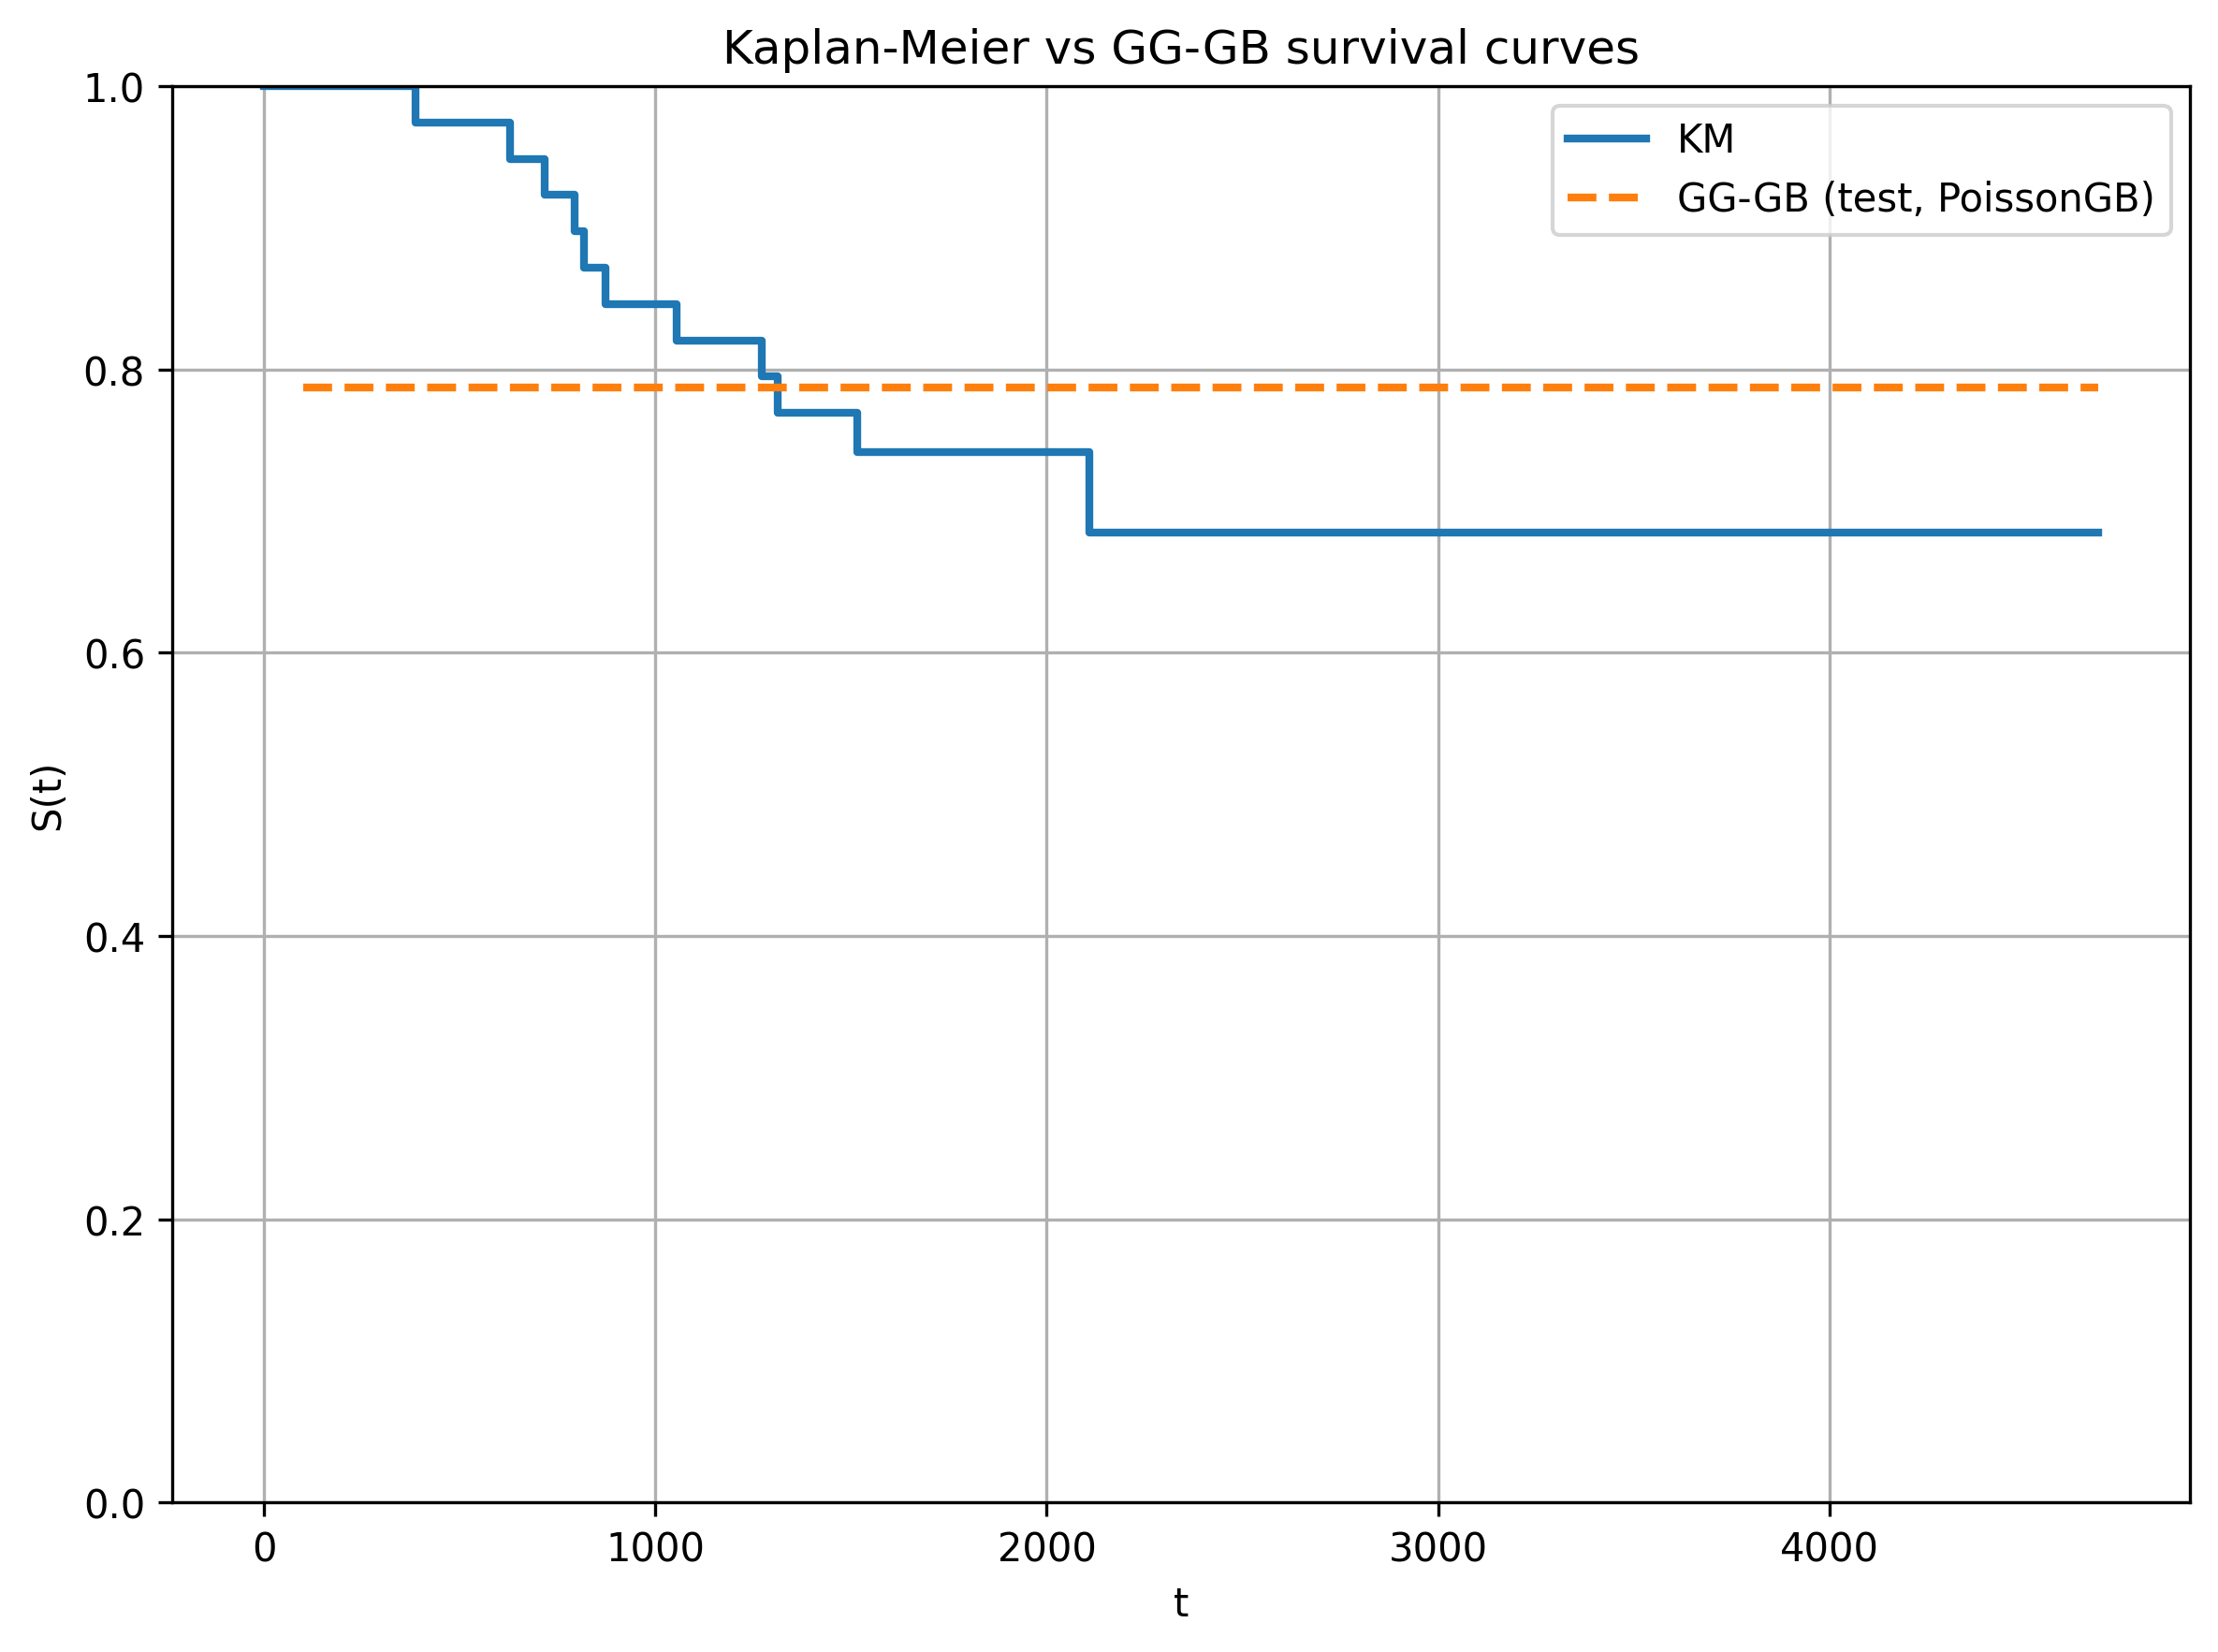
\includegraphics[width=\textwidth]{images/survival_curve_ggkm_testset_boost_poisson.png}
%         \caption{Boosted Poisson}
%     \end{subfigure}
%     \hfill
%     \begin{subfigure}{0.47\textwidth}
%         \centering
%         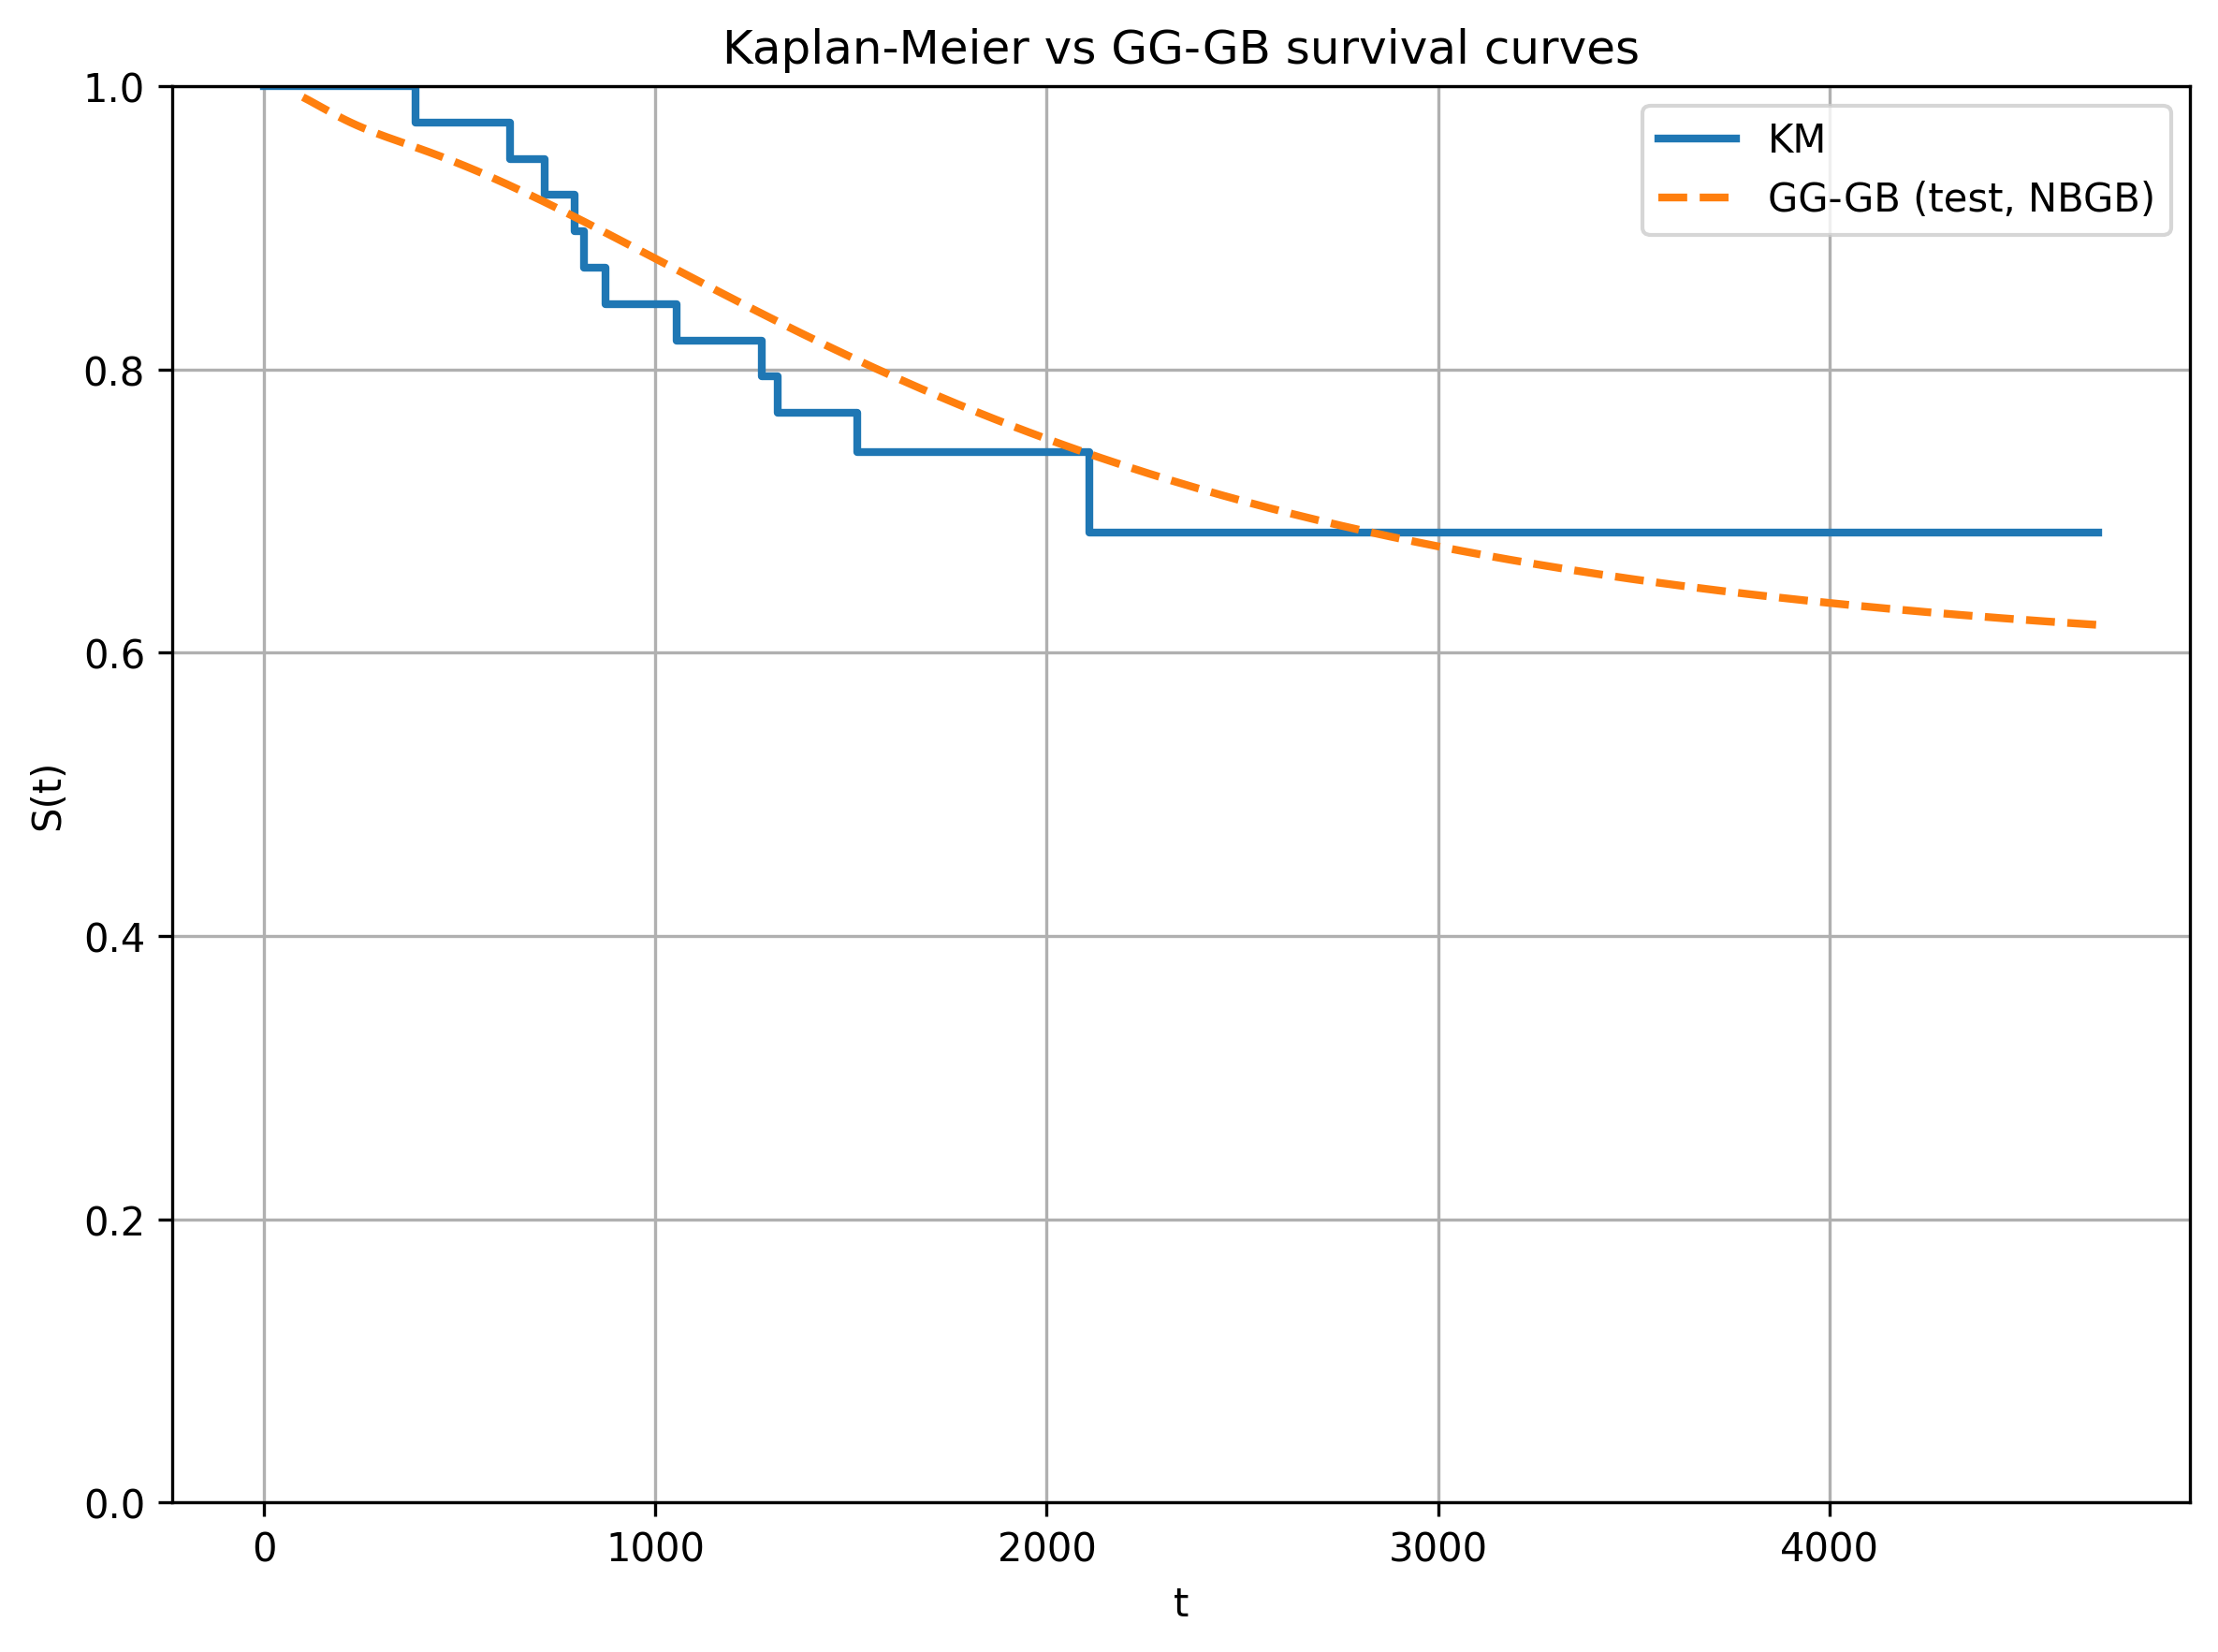
\includegraphics[width=\textwidth]{images/survival_curve_ggkm_testset_boost_bn.png}
%         \caption{Boosted Negative Binomial}
%     \end{subfigure}

%     \caption{Kaplan--Meier survival curves for the melanoma test set, comparing the GG-KM models under different distributions.}
%     \label{fig:melanoma_km_ggkm}
% \end{figure}

% Inicialmente, assim como foi feito com os dados simulados, foi realizada a comparação entre
% a curva de sobrevivência estimada pelo modelo proposto e o estimador de Kaplan-Meier, conforme apresentado
% na Figura~\ref{fig:melanoma_km_ggkm}. Como pode ser observado a partir da figura, há de fato indícios de que
% o modelo está conseguindo capturar adequadamente a fração de cura presente nos dados.

% \begin{figure}[htb]
%     \centering
%     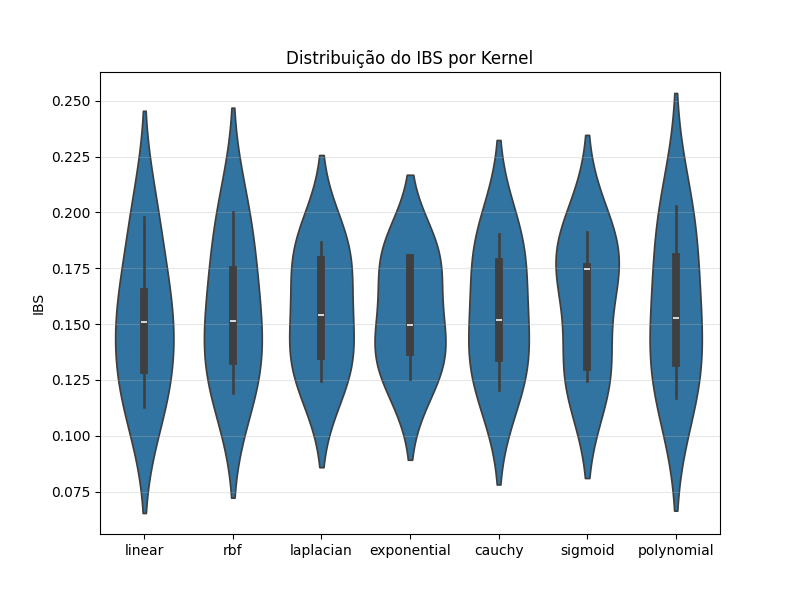
\includegraphics[width=0.6\textwidth]{images/melanoma_violin_ibs_em.png}
%     \caption{Distribuição do IBS em relação a cada kernel.}
%     \label{fig:melanoma_violin_ibs}
% \end{figure}

% \begin{figure}[htb]
%     \centering
%     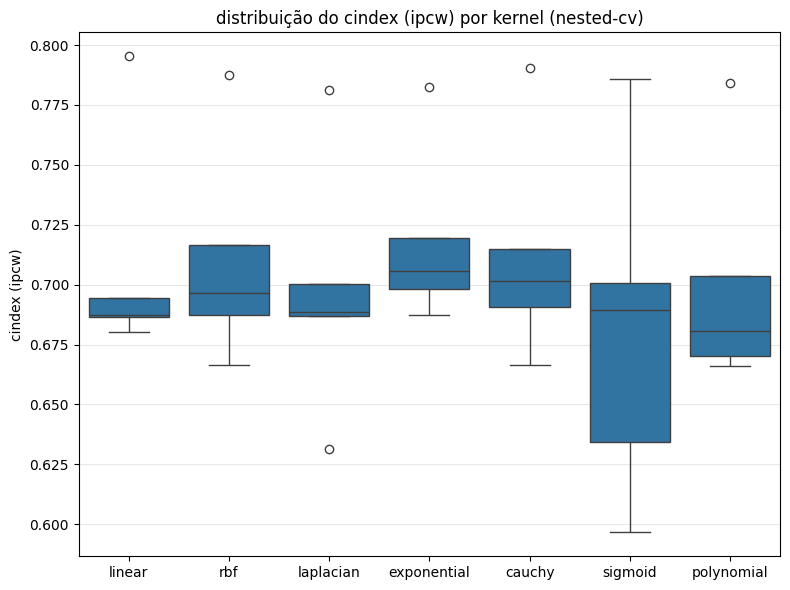
\includegraphics[width=0.6\textwidth]{images/boxplot_cindex_poisson.png}
%     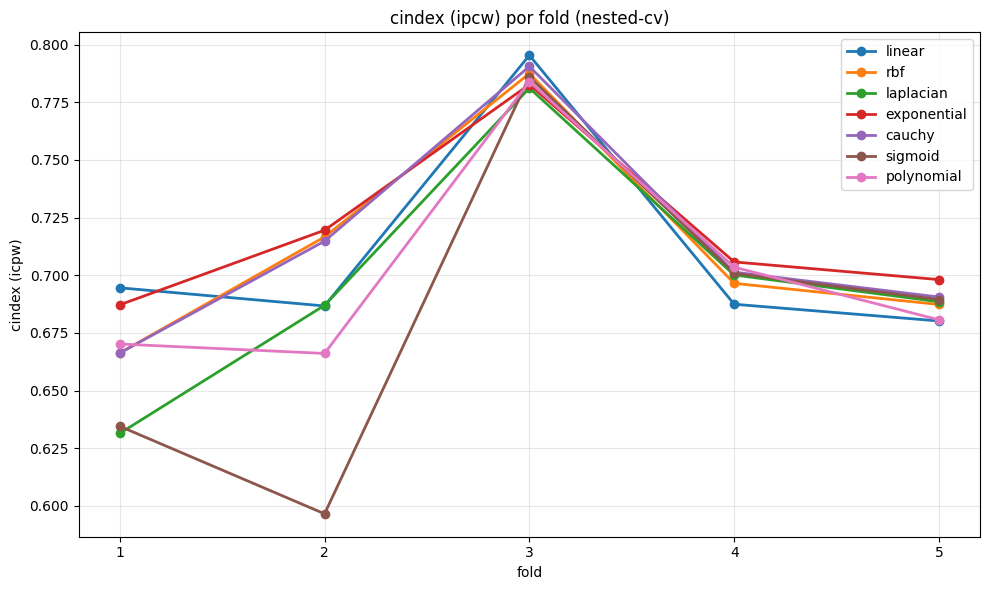
\includegraphics[width=0.6\textwidth]{images/nestedcv_poisson_cindex.png}
%     \caption{Distribuição do IBS em relação a cada kernel.}
%     \label{fig:melanoma_violin_ibs}
% \end{figure}

% Na Figura~\ref{fig:melanoma_violin_ibs}, pode-se observar a variação do desempenho do modelo GG-KM para
% cada kernel, com base na distribuição do IBS. Nota-se que o kernel cauchy, embora tenha alcançado
% um dos menores valores de IBS, foi também o que apresentou maior variabilidade nessa métrica. Os kernels
% linear e gaussiano apresentaram desempenhos bastante semelhantes entre si. De forma análoga, os kernels
% laplaciano e exponencial também exibiram resultados próximos, destacando-se por apresentarem menor
% variabilidade, embora não tenham atingido os menores valores de IBS. Por fim, os kernels sigmoid
% e polinomial também apresentaram comportamento semelhante, tanto em termos de nível quanto de dispersão do
% erro.

\begin{table}[ht]
\centering
\footnotesize
\setlength{\tabcolsep}{3pt}
\caption{Resultados do IBS médio, C-index médio, AUC médio e respectivos desvios padrão para cada kernel no conjunto de dados Melanoma, juntamente com o tempo de execução para cada distribuição de $N$.}
\label{tab:melanoma_kernels}

\begin{tabular}{
>{\centering\arraybackslash}p{2.8cm}
>{\centering\arraybackslash}p{1.4cm}
>{\centering\arraybackslash}p{1.5cm}
ccccccc
}
\toprule
$N$ & Time (min) & Métrica &
linear &
exponential &
cauchy &
rbf &
laplacian &
polynomial &
sigmoid \\
\midrule

\multirow{6}{*}{Poisson}
& \multirow{6}{*}{45.90}
& IBS
& 0.16519
& 0.16203
& 0.16564
& 0.16363
& 0.16002
& 0.17562
& 0.16214 \\

&
& DP IBS
& 0.02590
& 0.01918
& 0.02393
& 0.02289
& 0.02066
& 0.02836
& 0.01591 \\

&
& C-index
& 0.68563
& 0.71525
& 0.69617
& 0.69732
& 0.71008
& 0.64992
& 0.71090 \\

&
& DP C-index
& 0.09385
& 0.09151
& 0.09341
& 0.08980
& 0.09786
& 0.13254
& 0.08985 \\

&
& AUC
& 0.81078
& 0.69441
& 0.73703
& 0.69553
& 0.70275
& 0.72194
& 0.68404 \\

&
& DP AUC
& 0.05056
& 0.06351
& 0.05106
& 0.07890
& 0.03746
& 0.05533
& 0.06143 \\

\midrule

\multirow{6}{*}{\shortstack[c]{Binomial Negativa\\com $\phi$ estimado}}
& \multirow{6}{*}{68.46}
& IBS
& 0.16917
& 0.16203
& 0.16178
& 0.16131
& 0.15862
& 0.16293
& 0.16146 \\

&
& DP IBS
& 0.02834
& 0.01916
& 0.02149
& 0.02114
& 0.02023
& 0.01676
& 0.01885 \\

&
& C-index
& 0.70356
& 0.71488
& 0.70945
& 0.71009
& 0.71037
& 0.69918
& 0.70507 \\

&
& DP C-index
& 0.08676
& 0.09212
& 0.09106
& 0.08934
& 0.09651
& 0.08920
& 0.09043 \\

&
& AUC
& 0.76203
& 0.69459
& 0.71587
& 0.69384
& 0.69346
& 0.70382
& 0.69977 \\

&
& DP AUC
& 0.03687
& 0.06344
& 0.03678
& 0.06031
& 0.02794
& 0.04479
& 0.06095 \\

\midrule

\multirow{6}{*}{Bernoulli}
& \multirow{6}{*}{291.26}
& IBS
& 0.16742
& 0.15948
& 0.16378
& 0.16364
& 0.15948
& 0.16393
& 0.16618 \\

&
& DP IBS
& 0.03358
& 0.02212
& 0.02159
& 0.02224
& 0.02068
& 0.02494
& 0.02017 \\

&
& C-index
& 0.68894
& 0.71595
& 0.70678
& 0.70468
& 0.70825
& 0.69844
& 0.69138 \\

&
& DP C-index
& 0.09148
& 0.09836
& 0.08755
& 0.09047
& 0.09794
& 0.09558
& 0.09720 \\

&
& AUC
& 0.83980
& 0.70202
& 0.70563
& 0.71164
& 0.70229
& 0.73775
& 0.66067 \\

&
& DP AUC
& 0.05087
& 0.03374
& 0.05358
& 0.05173
& 0.05187
& 0.05418
& 0.08896 \\

\midrule

\multirow{6}{*}{Binomial}
& \multirow{6}{*}{86.60}
& IBS
& 0.16066
& 0.16184
& 0.16443
& 0.16231
& 0.15826
& 0.16660
& 0.15705 \\

&
& DP IBS
& 0.01896
& 0.01983
& 0.02368
& 0.02268
& 0.02017
& 0.02120
& 0.02004 \\

&
& C-index
& 0.67872
& 0.71194
& 0.69677
& 0.70904
& 0.70746
& 0.29430
& 0.72794 \\

&
& DP C-index
& 0.09758
& 0.09374
& 0.09404
& 0.09510
& 0.10155
& 0.36978
& 0.09003 \\

&
& AUC
& 0.54146
& 0.71091
& 0.71598
& 0.71328
& 0.66655
& 0.60220
& 0.70422 \\

&
& DP AUC
& 0.04792
& 0.06211
& 0.05637
& 0.07016
& 0.09270
& 0.12809
& 0.06074 \\

\bottomrule
\end{tabular}
\end{table}

\begin{table}[ht]
\centering
\footnotesize
\setlength{\tabcolsep}{5pt}
\caption{Resultados do IBS médio, C-index médio, AUC médio e respectivos desvios padrão para as abordagens de boosting e bagging no conjunto de dados Melanoma, juntamente com os respectivos tempos de execução.}
\label{tab:melanoma_ensemble}

\begin{tabular}{
>{\centering\arraybackslash}p{2.5cm}
>{\centering\arraybackslash}p{1.8cm}
>{\centering\arraybackslash}p{2.5cm}
>{\centering\arraybackslash}p{2.2cm}
cc
}
\toprule
$N$ & Tempo (min) & Abordagem & Métrica & Média & DP \\
\midrule

\multirow{6}{*}{Bernoulli}
& \multirow{3}{*}{3766.15}
& \multirow{3}{*}{Boosting}
& IBS
& 0.20606
& 0.06084 \\

&
&
& C-index
& 0.60949
& 0.05800 \\

&
&
& AUC
& 0.91526
& 0.04285 \\

\cmidrule{2-6}

&
\multirow{3}{*}{616.70}
& \multirow{3}{*}{Bagging}
& IBS
& 0.16184
& 0.02144 \\

&
&
& C-index
& 0.70700
& 0.10220 \\

&
&
& AUC
& 0.69115
& 0.03826 \\

\midrule

\multirow{3}{*}{Poisson}
& \multirow{3}{*}{4737.75}
& \multirow{3}{*}{Boosting}
& IBS
& 0.19676
& 0.03105 \\

&
&
& C-index
& 0.46930
& 0.23929 \\

&
&
& AUC
& 0.78523
& 0.14891 \\

\midrule

\multirow{3}{*}{\shortstack[c]{Binomial Negativa\\com $\phi$ estimado}}
& \multirow{3}{*}{5867.78}
& \multirow{3}{*}{Boosting}
& IBS
& 0.20688
& 0.05000 \\

&
&
& C-index
& 0.63721
& 0.05803 \\

&
&
& AUC
& 0.88976
& 0.07179 \\

\midrule

\multirow{3}{*}{Binomial}
& \multirow{3}{*}{4384.03}
& \multirow{3}{*}{Boosting}
& IBS
& 0.20493
& 0.04882 \\

&
&
& C-index
& 0.62684
& 0.02914 \\

&
&
& AUC
& 0.90809
& 0.05775 \\

\bottomrule
\end{tabular}
\end{table}

% A Tabela~\ref{tab:melanoma_kernels} resume esses resultados ao apresentar o IBS médio e seu respectivo
% desvio padrão para cada kernel. Observa-se que o kernel linear apresentou o menor IBS médio, indicando o
% melhor desempenho preditivo global nesse conjunto de dados, seguido de perto pelos kernels exponential e polynomial.

% Embora o kernel cauchy tenha apresentado alguns bons resultados, seu IBS médio mais elevado
% e maior variabilidade indicam menor estabilidade no processo de estimação. Por outro lado, o kernel
% exponential se destaca por combinar desempenho preditivo próximo ao melhor observado com a menor dispersão
% entre todos os kernels avaliados, sugerindo maior robustez. De modo geral, os resultados indicam que, para o
% conjunto de dados Melanoma, estruturas mais simples ou moderadamente flexíveis parecem ser suficientes para
% capturar adequadamente a dinâmica da sobrevivência e a fração de cura presente nos dados.
